\documentclass[main.tex]{subfiles}
\begin{document}
\chapter{Search Strategies}

Searching~\footnote{\url{https://en.wikipedia.org/wiki/Category:Search_algorithms}} is one of the most effective tools in algorithms. We  have seen them being widely applied in the field of artificial intelligence  to offer either exact or approximate solutions for complex problems such as puzzles, games, routing, scheduling, motion planning, navigation, and so on. On the spectrum of discrete problems, nearly every single one can be modeled as a searching problem together with enumerative combinatorics and \textbf{optimizations}. The searching solutions  serve as either naive baselines or even as the only existing solutions for some problems. Understanding common searching strategies as the main goal of this chapter along with  the search space of the problem lays the foundation of problem analysis and solving, it is just indescribably \textbf{powerful} and \textbf{important}! 



% In this chapter, we focus oncover the searching strategies from every possible aspect to make sure we understand it well and move on further. We

% This chapter, we assume the graph is connected graph. 

% The basic concepts will be explained in Section.~\ref{section_general_searching_strategies}.

% After this, we head out to apply these strategies given explicit data  structures for linear data structure in Sec.~\ref{section_linear_search}, Tree data structure in Sec.~\ref{section_tree_traversal} which are also called tree traversal algorithms, Graph data structures in Sec.~\ref{section_graph_search}. Along the applications, we will analyze them in terms of time and space complexity, completeness and optimality. 

% At the end, we will compare the difference of applying the searching strategies on the tree and graph data structures mainly how they would affect the completeness and optimaltities. 

\section{Introduction}
\label{section_linear_search}

Linear, tree-like data structures, they are all subsets of graphs, making graph searching universal to all searching algorithms. There are many searching strategies, and we only focus on a few decided upon the completeness of an algorithm--being absolutely sure to find an answer if there is one. 

Searching algorithms can be categorized into the following two types depending on if the domain knowledge is used to guide selection of tbe best path while searching:
\begin{enumerate}
    \item Uninformed Search: This set of searching strategies  normally are handled with basic and obvious problem definition and are not guided by estimation of how optimistic a certain node is. The basic algorithms include: Depth-first-Search(DFS), Breadth-first Search(BFS),  Bidirectional Search, Uniform-cost Search, Iterative deepening search, and so on. We choose to cover the first four. 
    \item Informed(Heuristic) Search: This set of searching strategies on the other hand, use additional domain-specific information to find a \textit{heuristic function} which estimates the cost of a solution from a node. Heuristics means ``serving to aid discovery''. Common algorithms seen here include: Best-first Search, Greedy Best-first Search, $A^{*}$ Search. And we only introduce Best-first Search. 
\end{enumerate}

% What types of searching algorithms are covered in this book?
% \begin{enumerate}
%     \item Combinatorial Search.
%     \item Backtracking.
%     \item Breath-First Search.
%     \item Depth-First Search
% \end{enumerate}

Following this introductory chapter, in Chapter.~\ref{chapter_search_problem_combinatorics}, we introduce combinatorial problems and its search space, and how to prune the search space to search more efficiently. 

Because the search space of a problem can either be of linear or tree structure--an implicit free tree, which makes the graph search a ``big deal'' in practice of problem solving. Compared with reduce and conquer, searching algorithms treat states and actions atomically: they do not consider any internal/optimal structure they might posses. We recap the \textbf{linear search} given its easiness and that we have already learned how to search in multiple linear data structures. 

\paragraph{Linear Search} As the naive and baseline approach compared with other searching algorithms, linear search, a.k.a sequential search, simply traverse the linear data structures sequentially and checking items until a target is found. It consists of a \texttt{for/while} loop, which gives as $O(n)$ as time complexity, and no extra space needed. For example, we search on list $A$ to find a target $t$:
\begin{lstlisting}[language=Python]
def linearSearch(A, t): #A is the array, and t is the target
    for i,v in enumerate(A):
        if A[i] == t:
            return i
    return -1
\end{lstlisting}

Linear Search is rarely used practically due to its lack of efficiency compared with other searching methods such as hashmap and binary search that we will learn soon.
\paragraph{Searching in Un-linear Space}
For the un-linear data structure, or search space comes from combinatorics, they are generally be a graph and sometimes be a rooted tree. Because mostly the search space forms a search tree, we introduce searching strategies on a search tree first, and then we specifically explore searching in a tree, recursive tree traversal, and search in a graph. 

\subsubsection{Generatics of Search Strategies}
Assume we know our state space, searching or state-space search is the process of searching through a state space for a solution by making explicit a sufficient portion of an implicit state-space graph, in the form of a search tree, to include a goal node. 

\paragraph{Nodes in Searching Process}
\begin{figure}[!ht]
    \centering
     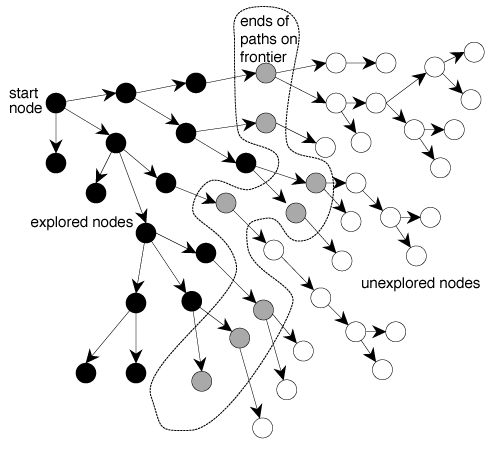
\includegraphics[width=0.9\columnwidth]{fig/searchsp.png}
    \caption{Graph Searching}
    \label{fig:search_sp}
\end{figure}
In the searching process, nodes in the targeting data structure can be categorized into three sets as shown in Fig.\ref{fig:search_sp} and we distinguish the state of a node--which set they are at with a color each.
\begin{itemize}
   \item Unexplored set--WHITE: initially all nodes in the graph are in the unexplored set, and we assign WHITE color. Nodes in this set have not yet being visited yet. 
    \item Frontier set--GRAY: nodes which themselves have been just discovered/visited and they are put into the \textit{frontier} set,  waiting to be expanded; that is to say their children or adjacent nodes (through outgoing edges) are about to be discovered and have not all been visited--not all being found in the frontier set yet. This is an intermediate state between WHITE and BLACK, which is ongoing, visiting but not yet completed. Gray vertex might have adjacent vertices of all three possible states.
%The set of nodes that are available for expansion at any given point is called the \textbf{frontier}.
    \item Explored set--BLACK: nodes have been fully explored after being in the frontier set; that is to say none of their children is not explored and being in the unexplored set. For black vertex, all vertices adjacent to them are nonwhite.% And the nodes that are expanded are distinguished as the \texttt{explored} set. 
 
\end{itemize}
All searching strategies follow the general tree search algorithm:
\begin{enumerate}
    \item At first, put the state node in the frontier set. 
\begin{lstlisting}
frontier = {S}
\end{lstlisting}
\item Loop through the frontier set, if it is empty then searching terminates. Otherwise, pick a node $n$ from frontier set:
\begin{enumerate}
    \item If $n$ is a goal node, then return solution
    \item Otherwise, generate all of $n$'s successor nodes and add them all to frontier set.
    \item Remove $n$ from frontier set.
\end{enumerate}
\end{enumerate}
Search process constructs a \textit{search tree} where the root is the start state. Loops in graph may cause the search tree to be infinite even if the state space is small. In this section, we only use either acyclic graph or tree for demonstrating the general search methods. In acyclic graph, there might exist multiple paths from source to a target. For example, the example shown in Fig.~\ref{} has multiple paths from to. Further in graph search section, we discuss how to handle cycles and explain single-path graph search.  Changing the ordering in the frontier set leads to different search strategies.


%%%%%%%%%%%%%%%Uninformed search strategies%%%%%%%%%%%%%%%%%%%
\section{Uninformed Search Strategies}
% in Search Tree

\begin{figure}[!ht]
    \centering
    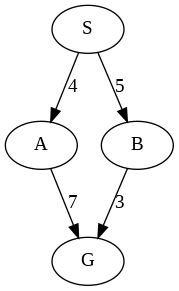
\includegraphics[width=0.3\columnwidth]{fig/ucs.png}
        \caption{Exemplary Acyclic Graph. }
    \label{fig:ucs}
\end{figure}
Through this section, we use Fig.~\ref{fig:ucs} as our exemplary graph to search on. The data structure to represent the graph is as:
\begin{lstlisting}[language=Python]
from collections import defaultdict
al = defaultdict(list)
al['S'] = [('A', 4), ('B', 5)]
al['A'] = [('G', 7)]
al['B'] = [('G', 3)]
\end{lstlisting}
%\subsection{Uninformed Search}

With uninformed search, we only know the goal test and the adjacent nodes, but without knowing which non-goal states are better. Assuming and limiting the state space to be a tree for now so that we won't worry about repeated states. 

There are generally two ways to order nodes in the frontier without domain-specific information:
\begin{itemize}
    \item Queue that nodes are first in and first out (FIFO) from the frontier set. This is called breath-first search.
    \item Stack that nodes are last in but first out (LIFO) from the frontier set. This is called depth-first search. 
    \item Priority queue that nodes are sorted increasingly in the path cost from source to each node from the frontier set. This is called Uniform-Cost Search.
\end{itemize}
%%%%%%%%%%%%%%%%%%BFS%%%%%%%%%%%%%%%%%%%%%%%
\subsection{Breath-first Search}
\begin{figure}[!ht]
    \centering
    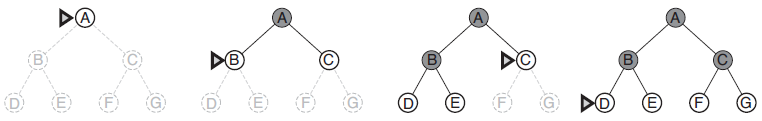
\includegraphics[width=0.96\columnwidth]{fig/general_breath_first_search.png}
        \caption{Breath-first search on a simple search tree. At each stage, the node to be expanded next is indicated by a marker. }
    \label{fig:breath_first_search_strategy}
\end{figure}
Breath-first search always expand the shallowest node in the frontier first, visiting nodes in the tree level by level as illustrated in Fig.~\ref{fig:breath_first_search_strategy}. Using $Q$ to denote the frontier set, the search process is explained:
\begin{lstlisting}[numbers=none]
Q=[A]
Expand A, add B and C into Q
Q=[B, C]
Expand B, add D and E into Q
Q=[C, D, E]
Expand C, add F and G into Q
Q=[D, E, F, G]
Finish expanding D
Q=[E, F, G]
Finish expanding E
Q=[F, G]
Finish expanding F
Q=[G]
Finish expanding G
Q=[]
\end{lstlisting}
The implementation can be done with a FIFO queue iteratively as:
\begin{lstlisting}[language=Python]
def bfs(g, s):
  q = [s]
  while q:
    n = q.pop(0)
    print(n, end = ' ')
    for v, _ in g[n]:
      q.append(v)
\end{lstlisting}
Call the function with parameters as \texttt{bfs(al, 'S')}, the output is as:
\begin{lstlisting}[numbers=none]
S A B G G 
\end{lstlisting}

%Instead of traversing the tree recursively deepening down each time, the alternative is to visit the nodes level by level, 

\paragraph{Properties} Breath-first search is \textbf{complete} because it can always find the goal node if it exists in the graph. It is also \textbf{optimal} given that all actions(arcs) have the same constant cost, or costs are positive and non-decreasing with depth. 

\paragraph{Time Complexity} We can clearly see that BFS scans each node in the tree exactly once. If our tree has $n$ nodes, it makes the time complexity $O(n)$. However, the search process can be terminated once the goal is found, which can be less than $n$. Thus we measure the time complexity by counting the number of nodes expanded while searching is running.  Assuming the tree has a branching factor $b$ at each non-leaf node and the goal node locates at depth $d$, we sum up the number of nodes from depth 0 to depth $d$, the total number of nodes expanded are:
\begin{align}
    n &= \sum_{i=0}^{d} b^{i} \\
    &= \frac{b^{d+1} -1}{b-1}
\end{align}
Therefore, we have a time complexity of $O(b^d)$. It is usually very slow to find solutions with a large number of steps because it must look at all shorter length possibilities first.%$in cases that we do not know the total nodes we estimate it with the branching factor, say $b$, as about how many children a node can have. In a binary tree, this would be 2, and with the depth $d$ of the tree, we get the time complexity as of $O(b^d)$.  
\paragraph{Space Complexity}
The space is measured in terms of the maximum size of frontier set during the search. In BFS, the maximum size is the number of nodes at depth $d$, making the $O(b^d)$ as the space complexity.

% However, because the different traversal ordering will result in different space usage. The BFS's implementation does not rely on stack but queue. The first implementation is more straightforward, the upper bound of space usage of \texttt{nodes\_same\_level} decides our memory space. Given a tree with branching factor $b$ and depth $d$, the lowest level will potentially have the most nodes, which has $O(b^d)$. 

% In the implementation that uses a queue, the analysis of the space usage is slight more obscure. We know it is decided by the maximum nodes storing in the \texttt{q} at one moment. Imagine the state change of the queue:
% \begin{lstlisting}[numbers=none]
% d = 0, [A]
% d = 1, process A, [B, C]
% d = 2, process B, [C, D, E], process C, [D, E, F, G]
% \end{lstlisting}
% This means the maximum space of our nodes still the same as our previous implementation, saving the nodes as large as the last level, which is $O(b^d)$. The implementation using the queue avoids the usage of the temporary list which is a slight improvement. 
%%%%%%%%%%%%%%%%%DFS%%%%%%%%%%%%%%%%%%%
\subsection{Depth-first Search}
\begin{figure}[!ht]
    \centering
     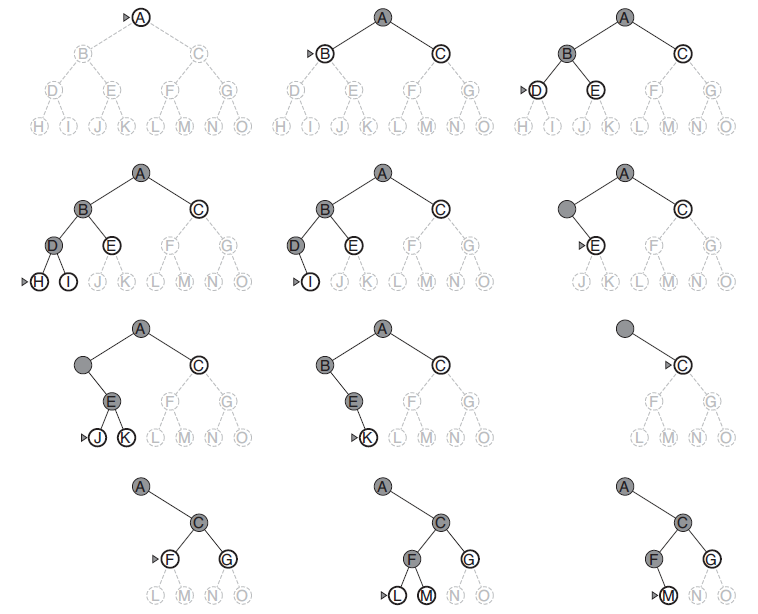
\includegraphics[width=0.96\columnwidth]{fig/general_depth_first_search.png}
    \caption{Depth-first search on a simple search tree. The unexplored region is shown in light gray. Explored nodes with no descendants in the frontier are removed from memory as node L disappears. Dark gray marks nodes that is being explored but not finished.   }
    \label{fig:depth_first_search_strategy}
\end{figure}
Depth-first search on the other hand always expand the deepest node from the frontier first. As shown in Fig.~\ref{fig:depth_first_search_strategy}, Depth-first search starts at the root node and continues branching down a particular path. Using $S$ to denote the frontier set which is indeed a stack, the search process is explained:
\begin{lstlisting}[numbers=none]
S=[A]
Expand A, add C and B into S
S=[C, B]
Expand B, add E and D into S
S=[C, E, D]
Expand D
S=[C, E]
Expand E
S=[C]
Expand C, add G and F into S
S=[C, G, F]
Expand F
S=[C, G]
Expand G
S=[C]
Expand C
S=[]
\end{lstlisting}
Depth-first can be implemented either recursively or iteratively. 
\paragraph{Recursive Implementation}In the recursive version, the recursive function keeps calling the recursive function itself to expand its adjacent nodes. Starting from a source node, it always deepen down the path until a leaf node is met and then it backtrack to expand its other siblings (or say other adjacent nodes). The code is as:
\begin{lstlisting}[language=Python]
def dfs(g, vi):
  print(vi, end=' ')
  for v, _ in g[vi]:   
    dfs(g, v)
\end{lstlisting}
Call the function with parameters as \texttt{dfs(al, 'S')}, the output is as:
\begin{lstlisting}[numbers=none]
S A G B G  
\end{lstlisting}
\paragraph{Iterative Implementation} According to the definition, we can implement DFS with LIFO \texttt{stack} data structure. The code is similar to that of BFS other than using different data structure from the frontier set.
\begin{lstlisting}[language=Python]
def dfs_iter(g, s):
  stack = [s]
  while stack:
    n = stack.pop()
    print(n, end = ' ')
    for v, _ in g[n]:
      stack.append(v)
\end{lstlisting}
Call the function with parameters as \texttt{dfs\_iter(al, 'S')}, the output is as:
\begin{lstlisting}[numbers=none]
S B G A G 
\end{lstlisting}
We observe that the ordering is not exactly the same as of the recursive counterpart. To keep the ordering consistent, we simply need to add the adjacent nodes in reversed order. In practice, we replace \texttt{$g[n]$} with \texttt{$g[n][::-1]$}.

\paragraph{Properties} DFS may not terminate without a fixed depth bound to limit the amount of nodes that it expand. DFS is \textbf{not complete} because it always deepens the search and in some cases the supply of nodes even within the cutting off fixed depth bound can be infinitely. DFS is \textbf{not optimal}, in our example, of our goal node is C, it goes through nodes A, B, D, E before it finds node C. While, in the BFS, it only goes through nodes A and C. However, when we are lucky, DFS can find long solutions quickly.

\paragraph{Time and Space Complexity} 
For DFS, it might need to explore all nodes within  graph to find the target, thus its worst case time and space complexity is not decided upon by the depth of the goal, but the total depth of the graph, $m$ instead. The time complexity of DFS is $O(b^m)$.

The stack will at most stores  a single path from the root to a leaf node (goal node) along with the  remaining unexpanded sibling nodes for each node on the path. Therefore, the space that needed for DFS is $O(bm)$. In most cases, the branching factor is a constant, which makes the space complexity be mainly influenced by the depth of the search tree. Obviously, DFS has great efficiency in space, which is why it is adopted as the basic technique in many areas of computer science, such as solving constraint satisfaction problems(CSPs). The backtracking technique we are about to introduce even further  optimizes the space complexity on the basis of DFS.

\subsection{Uniform-Cost Search(UCS)}
When a priority queue is used to order nodes measured by the path cost of each node to the root  in the frontier, this is called uniform-cost search, aka  Cheapest First Search. In UCS, frontier set is expanded only in the direction which requires the minimum cost to travel to from root node. UCS only terminates when a path has explored the goal node, and this path is the cheapest path among all paths that can reach to the goal node from the initial point.  When UCS is applied to find shortest path in a graph, it is called Dijkstra's Algorithm. 

We demonstrate the process of UCS with the example shown in Fig.~\ref{fig:ucs}.

Here, our source is `S', and the goal is `G'. We are set to find a path from source to goal with minimum cost. The process is shown as:
\begin{lstlisting}[numbers=none]
Q = [(0, S)]
Expand S, add A and B
Q = [(4, A), (5, B)]
Expand A, add G
Q = [(5, B), (11, G)]
Expand B, add G
Q = [(8, G), (11, G)]
Expand G, goal found, terminate.
\end{lstlisting}
And the Python source code is:
\begin{lstlisting}[language=Python]
import heapq
def ucs(graph, s, t):
  q = [(0, s)] # initial path with cost 0
  while q:
    cost, n = heapq.heappop(q)
    # Test goal
    if n == t:
      return cost
    else:
      for v, c in graph[n]:
        heapq.heappush(q, (c + cost, v))
  return None
\end{lstlisting}
\paragraph{Properties} Uniformed-Cost Search is \textbf{complete} as a similar search strategy compared with breath-first search(using queue). It is optimal even if there exist negative edges. 

\paragraph{Time and Space Complexity}  Similar to BFS, both the worst case time and space complexity is $O(b^d)$. When all edge costs are $c$, and $C^{*}$ is the best goal path cost, the time and space complexity can be more precisely represented as $O(b^{C^{*}/c})$.
\subsection{Iterative-Deepening Search}
Iterative-Deepening Search(IDS) is a modification on top of DFS, more specifically depth limited DFS(DLS); as the name suggests, IDS sets a maximum depth as a ``depth bound'', and it calls DLS as a subroutine looping from depth zero to maximum depth to expand nodes just as DFS will do and it only does goal test for nodes at the testing depth.

Using the graph in Fig.~\ref{fig:ucs} as an example. The process is shown as:
\begin{lstlisting}[numbers=none]
maxDepth = 3

depth = 0: S = [S]
Test S, goal not found

depth = 1: S =[S]
Expand S, S = [B, A]
Test A, goal not found
Test B, goal not found

depth  = 2: S=[S]
Expand S, S=[B, A]
Expand A, S=[B, G]
Test G, goal found, STOP
\end{lstlisting}
The implementation of the DLS goes easier with recursive DFS, we use a count down to variable \texttt{maxDepth} in the function, and will only do goal testing util this variable reaches to zero. The code is as:
\begin{lstlisting}[language=Python]
def dls(graph, cur, t, maxDepth):
  # End Condition
  if maxDepth == 0:
    if cur == t:
      return True
  if maxDepth < 0:
    return False

  # Recur for adjacent vertices
  for n, _ in graph[cur]:
    if dls(graph, n, t, maxDepth - 1):
      return True
  return False
\end{lstlisting}
With the help of function \texttt{dls}, the implementation of DLS is just an iterative call to the subroutine:
\begin{lstlisting}[language=Python]
def ids(graph, s, t, maxDepth):
  for i in range(maxDepth):
    if dls(graph, s, t, i):
      return True
  return False
\end{lstlisting}
\paragraph{Analysis} It appears to us that we are undermining the efficiency of the original DFS since the algorithm ends up visiting top level nodes of the goal multiple times. However, it is not as expensive as it seems to be, since in a tree most of the nodes are in the bottom levels. If the goal node locates at the bottom level, DLS will not have an obvious efficiency decline. But if the goal locates on topper levels on the right side of the tree, it avoids to visit all nodes across all depths on the left half first and then be able to find this goal node.
\paragraph{Properties} Through the depth limited DFS, IDS has advantages of DFS: 
\begin{itemize}
    \item Limited space linear to the depth and branching factor, giving $O(bd)$ as space complexity.
    \item In practice, even with redundant effort, it still finds longer path more quickly than BFS does.
\end{itemize}
By iterating through from lower to higher depth, IDS has advantages of BFS, which comes with \textbf{completeness} and \textbf{optimality} stated the same as of BFS. 
\paragraph{Time and Space Complexity}
The space complexity is the same as of BFS, $O(bd)$. The time complexity is slightly worse than BFS or DFS due to the repetitive visiting nodes on top of the search tree but it still has the same worst case exponential time complexity, $O(b^d)$. 
%%%%%%%%%%%%%%%%Bidirectional Search%%%%%%%%%%%%%%%%%%%%%%%%%%%%%%
\subsection{Bidirectional Search**}
\begin{figure}[!ht]
    \centering
    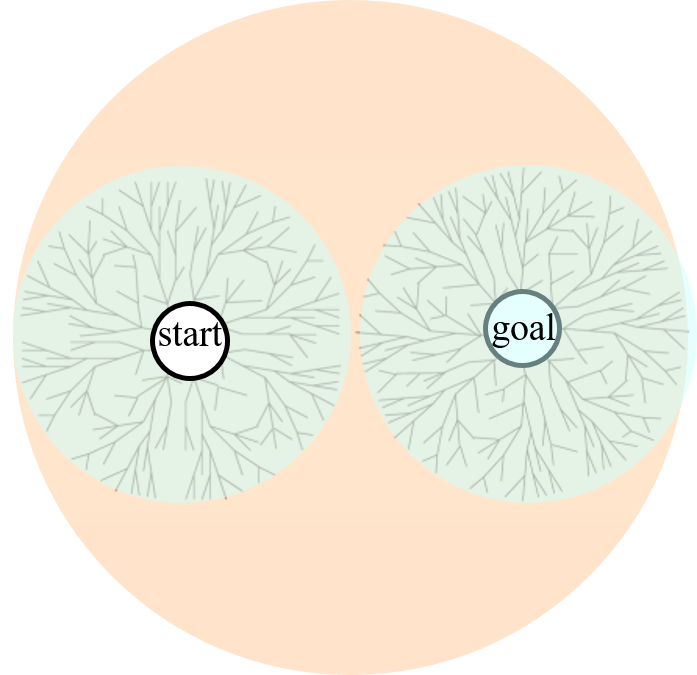
\includegraphics[width=0.5\columnwidth]{fig/bidrectional_search.png}
        \caption{Bidirectional search. }
    \label{fig:bidirectional_search}
\end{figure}
Bidirectional search applies breadth-first search from both the start and the goal node, with one BFS from start moving forward and one BFS from the goal moving backward until their frontiers meet. This process is shown in Fig.~\ref{fig:bidirectional_search}. As we see, each BFS process only visit $O(b^{d/2})$ nodes comparing with one single BFS that visits $O(b^d)$ nodes. This will improve both the time and space efficiency by $b^{d/2}$ times compared with vanilla BFS. 
\paragraph{Implementation} Because the BFS that starts from the goal needs to move backwards, the easy way to do this is to create another copy of the graph wherein each edge has opposite direction compared with the original. By creating a reversed graph, we can use a forward BFS from the goal. 

We apply level by level BFS instead of updating the queue one node by one node. For better efficiency of the intersection of the frontier set from both BFS, we use \texttt{set} data structure instead of simply a \texttt{list} or a FIFO queue. 

Use Fig.~\ref{fig:ucs} as an example, if our source and goal is `S' and `G' respectively, if we proceed both  BFS simultaneously, the process looks like this:
\begin{lstlisting}[numbers=none]
qs = ['S']
qt = ['G']
Check intersection, and proceed
qs = ['A', 'B']
qt = ['A', 'B']
Check intersection, frontier meet, STOP
\end{lstlisting}
No process in this case, however, the above process will end up missing the goal node if we change our goal to be `A'. This process looks like:
\begin{lstlisting}[numbers=none]
qs = ['S']
qt = ['A']
Check intersection, and proceed
qs = ['A', 'B']
qt = ['S']
Check intersection, and proceed
qs = ['G']
qt = []
STOP
\end{lstlisting}
This because for source and goal nodes that has a shortest path with even length, if we proceed the search process simultaneously, we will always end up missing the intersection. Therefore, we process each BFS iteratively--one at a time to avoid such troubles. 

The code for one level at a time BFS with \texttt{set} and for the intersection check is as:
\begin{lstlisting}[language=Python]
def bfs_level(graph, q, bStep):
  if not bStep:
    return q
  nq = set()
  for n in q:
    for v, c in graph[n]:
      nq.add(v)
  return nq

def intersect(qs, qt):
  if qs & qt: # intersection 
    return True
  return False
\end{lstlisting}
The main code for bidirectional search is as:
\begin{lstlisting}[language=Python]
def bis(graph, s, t):
  # First build a graph with opposite edges 
  bgraph = defaultdict(list)
  for key, value in graph.items():
    for n, c in value:
      bgraph[n].append((key, c))
  # Start bidirectional search
  qs = {s}
  qt = {t}
  step = 0
  while qs and qt:
    if intersect(qs, qt):
      return True
    qs = bfs_level(graph, qs, step%2 == 0)
    qt = bfs_level(bgraph, qt, step%2 == 1)
    step = 1 - step
  return False
\end{lstlisting}
\subsection{Summary}
\begin{table}[!ht]
\begin{small}
\centering
\noindent\captionof{table}{ Performance of Search Algorithms on Trees or Acyclic Graph}
 \noindent \begin{tabular}{|p{0.2\columnwidth}|p{0.15\columnwidth}|p{0.15\columnwidth}|p{0.15\columnwidth}|p{0.15\columnwidth}| }
  \hline
Method & Complete & Optimal & Time & Space   \\ \hline
BFS  & Y& Y, if & $O(b^d)$ & $O(b^d)$ \\\hline
UCS  &Y & Y & $O(C^{*}/c)$ & $O(C^{*}/c)$\\ \hline
DFS & N & N & $O(b^m)$ & $O(bm)$\\ \hline
IDS & Y & Y, if & $O(b^d)$ & $O(bd)$\\ \hline
Bidireactional Search & Y& Y, if& $O(b^{d/2})$ & $O(b^{d/2})$\\ \hline
\end{tabular}
  \label{tab:performance of searching strategy}
  \end{small}
\end{table}
Using $b$ as branching factor, $d$ as the depth of the goal node, and $m$  is the maximum graph depth. The properties and complexity for the five uninformed search strategies are summarized in Table.~\ref{tab:performance of searching strategy}.

 


 
 %%%%%%%%%%%%%%%%%Graph Search%%%%%%%%%%%%%%%%%%%%%%%%%%%%%%%
\section{Graph Search}
\paragraph{Cycles}
This section is devoted to discuss more details about two search strategies--BFS and DFS in more general graph setting. In the last section, we just assumed our graph is either a tree or acyclic directional graph. In more general real-world setting, there can be cycles within a graph which will lead to infinite loops of our program. 
\paragraph{Print Paths} Second, we talked about the paths, but we never discuss how to track all the paths. In this section, we would like to see how we can track paths first, and then with the tracked paths, we detect cycles to avoid getting into infinite loops. 
\paragraph{More Efficient Graph Search}
Third, the last section is all about tree search, however, in a large graph, this is not efficient by visiting some nodes multiple times if they happen to be on the multiple paths between the source and any other node in the graph. Usually, depends on the application scenarios, graph search which remembers already-expanded nodes/states in the graph and avoids expanding again by checking any about to be expanded node to see if it exists in frontier set or the explored set. This section, we introduce graph search that suits for general purposed graph problems. 
% \paragraph{Handle Cycles} In this section, we assumed our graph is either a tree or acyclic directional graph. When there are cycles, we have to track the path and avoid cycles, which you will see more details in Section Graph Search. 
% \paragraph{Graph Search}
% This section is all about tree search, however, in a large graph, this is not efficient by visiting some nodes multiple times if they happen to be on the multiple paths between the source and any other node in the graph. Usually, depends on the application scenarios, graph search which remembers already-expanded nodes/states in the graph and avoids expanding again by checking any about to be expanded node to see if it exists in frontier set or the explored set. Check Section. Graph search for more details. 
% \paragraph{Print Paths} We have known that the uniformed search were all doing tree based search, but we never try to track all the paths, which we would like to resolve in the next section. 
% In this Chapter, we expand the BFS and DFS tree searching strategy on a graph which is more general. 

%For convenience, we use two sets: \textit{explored set} and \textit{frontier set} to distinguish vertices that have been finished exploring and vertices that are being explored. This make three different states between all vertices in the searching process:
\paragraph{Visiting States} 
We have already explained that we can use three colors: WHITE, GREY, and BLACK to denote nodes within the unexpanded, frontier, and explored set, respectively. We are doing so to avoid the hassles of tracking three different sets, with visiting state, it is all simplified to a color check. We define a \texttt{STATE} class for convenience.
% Because in graph, it is reasonable to expect it contains cycles. In our example, we have a cycle \texttt{[0, 1, 2, 0]} and \texttt{[1, 2, 3, 4, 1]} as shown in Fig.~\ref{fig:cyclic_graph_search_1}. Therefore, in the graph search, it is a necessity to avoid traversing a cycle which will make the program running nonstop. The solution is during the search process, we mark states for each vertex. 



\begin{lstlisting}[language=Python, numbers=none]
class STATE:
    white = 0
    gray = 1
    black = 2
\end{lstlisting}
\begin{figure}[!ht]
    \centering
     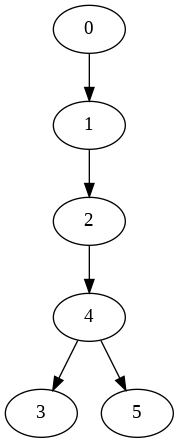
\includegraphics[width=0.25\columnwidth]{fig/free_tree.png}
     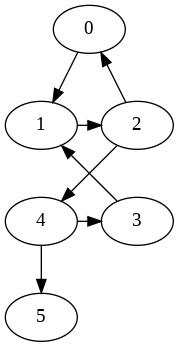
\includegraphics[width=0.25\columnwidth]{fig/directed_cyclic_graph.png}
      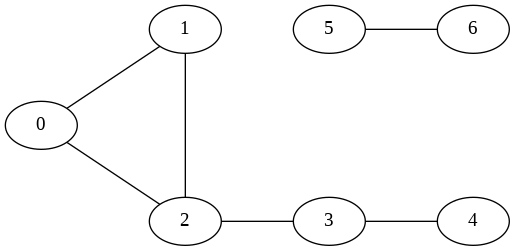
\includegraphics[width=0.25\columnwidth]{fig/undirected_cyclic_graph.png}
    \caption{Exemplary Graph: Free Tree, Directed Cyclic Graph, and Undirected Cyclic Graph.}
    \label{fig:graph_search_example}
\end{figure}
In this section, we use Fig.~\ref{fig:graph_search_example} as our exemplary graphs. Each's data structure is defined as:
\begin{itemize}
\item Free Tree:
\begin{lstlisting}[language=Python]
ft = [[] for _ in range(6)]
ft[0] = [1]
ft[1] = [2]
ft[2] = [4]
ft[4] = [3, 5]
\end{lstlisting}
    \item Directed Cyclic Graph:
    \begin{lstlisting}[language=Python]
dcg = [[] for _ in range(6)]
dcg[0] = [1]
dcg[1] = [2]
dcg[2] = [0, 4]
dcg[3] = [1]
dcg[4] = [3, 5]
\end{lstlisting}
\item Undirected Cyclic Graph
    \begin{lstlisting}[language=Python]
ucg = [[] for _ in range(6)]
ucg[0] = [1, 2]
ucg[1] = [0, 2, 3]
ucg[2] = [0, 1,  4]
ucg[3] = [1, 4]
ucg[4] = [2, 3, 5]
ucg[5] = [4]
\end{lstlisting}
\end{itemize}

% Then we introduce more searching strategies such as priority-first searching and give out more categorization. 

\paragraph{Search Tree} It is important to realize the Searching ordering is always forming a tree, this is terminologized as \textbf{Search Tree}. In a tree structure, the search tree is itself. In a graph, we need to figure out the search tree and it decides our time and space complexity. 


 
 %%%%%%%%%%%%%%%%%%%%%%%%%%%Graph Search%%%%%%%%%%%%%%%%%%%%%
\subsection{Depth-first Search in Graph}
In this section we will further the depth-first tree search and explore depth-first graph search to compare their properties and complexity.  
\subsubsection{Depth-first Tree Search} 

\paragraph{Vanilla Depth-first Tree Search} Our previous code slightly modified to suit for the new graph data structure works fine with the free tree in Fig.~\ref{fig:graph_search_example}. The code is as:
\begin{lstlisting}[language=Python]
def dfs(g, vi):
  print(vi, end=' ')
  for nv in g[vi]:   
    dfs(g, nv)
\end{lstlisting}
However, if we call it on the cyclic graph, \texttt{dfs(dcg, 0)}, it runs into stack overflow.

\paragraph{Cycle Avoiding Depth-first Tree Search} 
So, how to avoid cycles? We know the definition of a cycle is a closed path that has  at least one node that repeats itself; in our failed run, we were stuck with cycle [0, 1, 2, 0]. Therefore, let us add a \texttt{path} in the recursive function, and whenever we want to expand a node, we check if it forms a cycle or not by checking the membership of a candidate to nodes comprising the path.  We save all paths and the visiting ordering of nodes in two list: \texttt{paths} and \texttt{orders}. The recursive version of code is:
\begin{lstlisting}[language=Python]
def dfs(g, vi, path):
  paths.append(path)
  orders.append(vi)
  for nv in g[vi]:  
    if nv not in path: 
      dfs(g, nv, path+[nv])
  return 
\end{lstlisting}
Now we call function \texttt{dfs} for \texttt{ft}, \texttt{dcg}, and \texttt{ucg}, the \texttt{paths} and \texttt{orders} for each example is listed:
\begin{itemize}
    \item For the free tree and the directed cyclic graph, they have the same output. The \texttt{orders} are:
\begin{lstlisting}[numbers=none]
[0, 1, 2, 4, 3, 5]
\end{lstlisting}
    And the \texttt{paths} are:
\begin{lstlisting}[numbers=none]
[[0], [0, 1], [0, 1, 2], [0, 1, 2, 4], [0, 1, 2, 4, 3], [0, 1, 2, 4, 5]]
\end{lstlisting}
    \item For the undirected cyclic graph, \texttt{orders} are:
\begin{lstlisting}[numbers=none]
[0, 1, 2, 4, 3, 5, 3, 4, 2, 5, 2, 1, 3, 4, 5, 4, 3, 1, 5]
\end{lstlisting}
    And the \texttt{paths} are:
\begin{lstlisting}[numbers=none]
[[0],
[0, 1],
[0, 1, 2],
[0, 1, 2, 4],
[0, 1, 2, 4, 3],
[0, 1, 2, 4, 5],
[0, 1, 3],
[0, 1, 3, 4],
[0, 1, 3, 4, 2],
[0, 1, 3, 4, 5],
[0, 2],
[0, 2, 1],
[0, 2, 1, 3],
[0, 2, 1, 3, 4],
[0, 2, 1, 3, 4, 5],
[0, 2, 4],
[0, 2, 4, 3],
[0, 2, 4, 3, 1],
[0, 2, 4, 5]]
\end{lstlisting}
\end{itemize}
\begin{figure}[!ht]
    \centering
     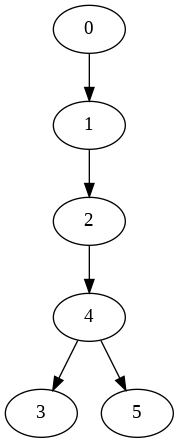
\includegraphics[width=0.2\columnwidth]{fig/free_tree.png}
    % 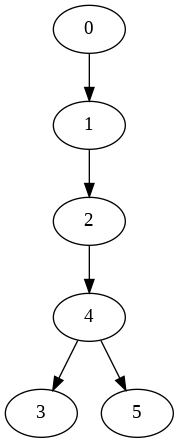
\includegraphics[width=0.15\columnwidth]{fig/free_tree.png}
      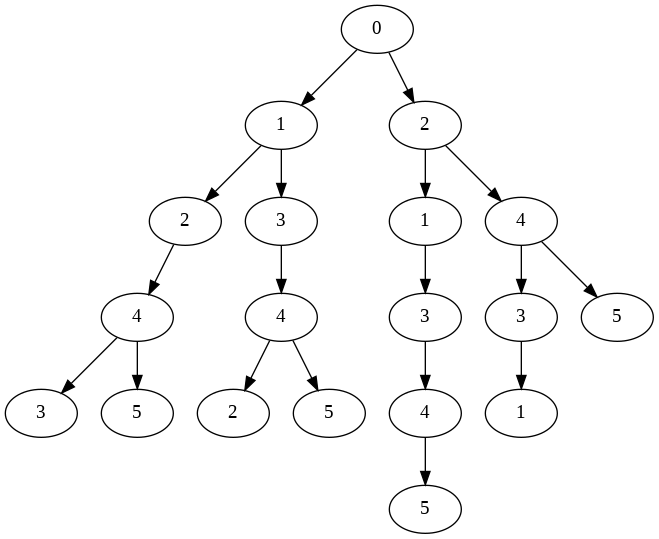
\includegraphics[width=0.75\columnwidth]{fig/search_tree_dfs.png}
    \caption{Search Tree for Exemplary Graph: Free Tree and Directed Cyclic Graph, and Undirected Cyclic Graph.}
    \label{fig:graph_search_example_search_tree}
\end{figure}

These paths mark the search tree, we visualize the search tree for each exemplary graph in Fig.~\ref{fig:graph_search_example_search_tree}. 

% \paragraph{Efficient Path Backtrace} Previously we save paths each as a list, the shared partial paths locating on top part of the search tree are repeating, such as partial path [0, 1, 2, 4] in our example, which wastes memory unnecessarily. We can save paths by saving all edges in the search tree

\subsubsection{Depth-first Graph Search}
 We see that from the above implementation, for a graph with only 6 nodes, we have been visiting nodes for a total of 19 times. A lot of nodes have been repeating. 1 appears 3 times, 3 appears 4 times, and so on. As we see the visiting order being represented with a \texttt{search tree} in Fig.~\ref{fig:graph_search_example_search_tree}, our complexity is getting close to $O(b^h)$, where $b$ is the branching factor and $h$ is the total vertices of the graph, marking the upper bound of the maximum depth that the search can traverse. If we simply want to search if a value or a state exists in the graph, this is insanely complicating the situation. What we do next is to avoid revisiting the same vertex again and again, we conquer this by tracking the visiting state of a node. 
 
 In the implementation, we only track the longest path--from source vertex to vertex that has no more unvisited adjacent vertices. 
\begin{lstlisting}[language=Python]
def dfgs(g, vi, visited, path):
  orders.append(vi)
  bEnd = True # node without unvisited adjacent nodes    
  for nv in g[vi]:  
    if nv not in visited: 
      if bEnd:
        bEnd = False
      visited.add(nv)
      dfgs(g, nv, visited, path + [nv])
  if bEnd:
    paths.append(path)
\end{lstlisting}
Now, we call this function with \texttt{ucg} as:
\begin{lstlisting}[language=Python]
paths, orders = [], []
dfgs(ucg, 0, set([0]), [0])
\end{lstlisting}
The output for \texttt{paths} and \texttt{orders} are:
\begin{lstlisting}[numbers=none]
([[0, 1, 2, 4, 3], [0, 1, 2, 4, 5]], [0, 1, 2, 4, 3, 5])
\end{lstlisting}
Did you notice that the depth-first graph search on the undirected cyclic graph shown in Fig.~\ref{fig:graph_search_example} has the same visiting order of nodes and same search tree as the free tree and directed cyclic graph in Fig.~\ref{fig:graph_search_example}?


\paragraph{Properties} The completeness of DFS depends on  the search space. If your search space is finite, then Depth-First Search is complete. However, if there are infinitely many alternatives, it might not find a solution. For example, suppose you were coding a path-search problem on city streets, and every time your partial path came to an intersection, you always searched the left-most street first. Then you might just keep going around the same block indefinitely.

The depth-first graph search is \textbf{nonoptimal} just as Depth-first tree search. For example, if the task is to find the shortest path from source 0 to target 2. The shortest path should be 0->2, however depth-first graph search will return 0->1->2. For the search tree using depth-first tree search, it can find the shortest path from source 0 to 2. However, it will explore the whole left branch starts from 1 before it finds its goal node on the right side. 

\paragraph{Time and Space Complexity}   For the depth-first graph search, we use aggregate analysis. The search process covers all edges, $|E|$ and vertices, $|V|$, which makes the time complexity as $O(|V|+|E|)$. For the space, it uses space $O(|V|)$ in the worst case to
store the stack of vertices on the current search path as well as the set of
already-visited vertices.

\subsubsection{Applications} Depth-first tree search is adopted as the basic workhorse of many areas of AI, such as solving CSP. Depth-first graph search is widely used to solve graph related tasks, such as Cycle Check, Topological sort, backtracking. 
% Let's call it as \texttt{recursive(al, 0, [0])}, and the output that indicates the visiting order of vertices will be:
% \begin{lstlisting}[numbers=none]
% 0 1 2 4 3 5 6 3 4 2 5 6 2 1 3 4 5 6 4 3 1 5 6 
% \end{lstlisting}
%  \begin{figure}[!ht]
%     \centering
%     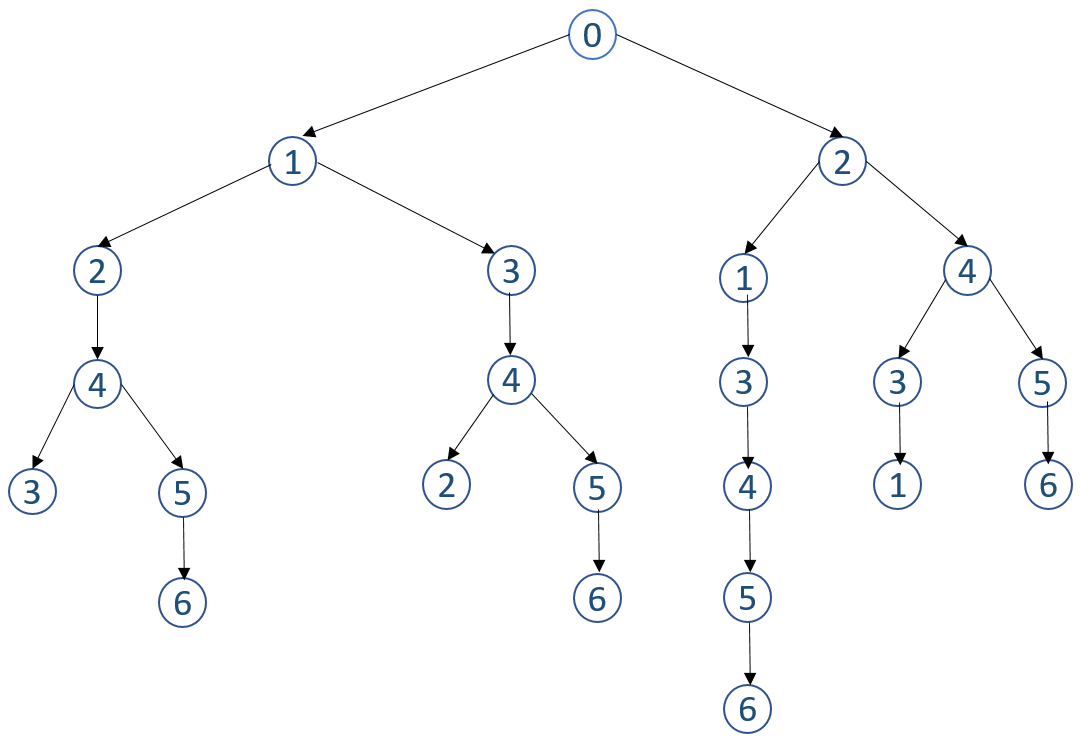
\includegraphics[width=0.9\columnwidth]{fig/depth_first_tree_search.png}
%     \caption{The search tree using depth-first tree search }
%     \label{fig:df_tree_search}
% \end{figure}
% \begin{figure}[!ht]
%     \centering
%     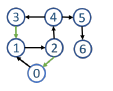
\includegraphics[width=0.5\columnwidth]{fig/free_tree_search.png}
%     \caption{The search tree using depth-first graph search.}
%     \label{fig:dfs_graph_search}
% \end{figure}
% And the following are all the paths comprise the search tree shown  in Fig.~\ref{fig:df_tree_search}.
% \begin{lstlisting}[language=Python]
% [0] [0, 1] [0, 1, 2] [0, 1, 2, 4] [0, 1, 2, 4, 3] [0, 1, 2, 4, 5] [0, 1, 2, 4, 5, 6] [0, 1, 3] [0, 1, 3, 4] [0, 1, 3, 4, 2] [0, 1, 3, 4, 5] [0, 1, 3, 4, 5, 6] [0, 2] [0, 2, 1] [0, 2, 1, 3] [0, 2, 1, 3, 4] [0, 2, 1, 3, 4, 5] [0, 2, 1, 3, 4, 5, 6] [0, 2, 4] [0, 2, 4, 3] [0, 2, 4, 3, 1] [0, 2, 4, 5] [0, 2, 4, 5, 6] 
% \end{lstlisting}

\begin{bclogo}[couleur = blue!30, arrondi=0.1,logo=\bccrayon,ombre=true]{Questions to ponder: } 
\begin{itemize}
\item Only track the longest paths.
\item How to trace the edges of the search tree?
\item Implement the iterative version of the recursive code.
\end{itemize}
\end{bclogo}

%%%%%%%%%%%%%%BFS%%%%%%%%%%%%%%%%%%%%%%%%
%%%%%%%%%%%%%%%%%%%%
\subsection{Breath-first Search in Graph}
We further breath-first tree search and explore breath-first graph search in this section to grasp better understanding of one of the most general search strategies. Because that BFS is implemented iteratively, the implementation in this section of sheds light to the iterative counterparts of DFS's recursive implementations from last section. 
\subsubsection{Breath-first Tree Search}
Similarly, out vanilla breath-first tree search shown in Section.~\ref{} will get stuck with the cyclic graph in Fig.~\ref{fig:graph_search_example}. 
\paragraph{Cycle Avoiding Breath-first Tree Search} We avoid cycles with similar strategy to DFS tree search that traces paths and checks membership of node. In BFS, we track paths by explicitly adding paths to the \texttt{queue}. Each time we expand from the frontier (queue), the node we need is the last item in the path from the queue. In the implementation, we only track the longest paths from the search tree and the visiting orders of nodes. The Python code is:
\begin{lstlisting}[language=Python]
def bfs(g, s):
  q = [[s]]
  paths, orders = [], []
  while q:
    path = q.pop(0)
    n = path[-1]
    orders.append(n)
    bEnd = True
    for v in g[n]:
      if v not in path:
        if bEnd:
          bEnd = False
        q.append(path + [v])
    if bEnd:
      paths.append(path)
  return paths, orders
\end{lstlisting}
Now we call function \texttt{bfs} for \texttt{ft}, \texttt{dcg}, and \texttt{ucg}, the \texttt{paths} and \texttt{orders} for each example is listed:
\begin{itemize}
    \item For the free tree and the directed cyclic graph, they have the same output. The \texttt{orders} are:
\begin{lstlisting}[numbers=none]
[0, 1, 2, 4, 3, 5]
\end{lstlisting}
    And the \texttt{paths} are:
\begin{lstlisting}[numbers=none]
[[0, 1, 2, 4, 3], [0, 1, 2, 4, 5]]
\end{lstlisting}
    \item For the undirected cyclic graph, \texttt{orders} are:
\begin{lstlisting}[numbers=none]
[0, 1, 2, 2, 3, 1, 4, 4, 4, 3, 3, 5, 3, 5, 2, 5, 4, 1, 5]
\end{lstlisting}
    And the \texttt{paths} are:
\begin{lstlisting}[numbers=none]
[[0, 2, 4, 5], [0, 1, 2, 4, 3], [0, 1, 2, 4, 5], [0, 1, 3, 4, 2], [0, 1, 3, 4, 5], [0, 2, 4, 3, 1], [0, 2, 1, 3, 4, 5]]
\end{lstlisting}
\end{itemize}
We can see the visiting orders of nodes are different from Depth-first tree search counterparts. However, the corresponding search tree for each graph in Fig.~\ref{fig:graph_search_example} is the same as of counterpart Depth-first Tree Search illustrated in Fig.~\ref{fig:graph_search_example_search_tree}. This highlights how different searching strategies differ by visiting ordering of nodes but not differ at the search-tree which depicts the search space.  




\paragraph{Applications} However, the Breath-first Tree Search and path tracing is extremely more costly compared with DFS counterpart. When our goal is to enumerate paths, go for the DFS. When we are trying to find shortest-paths, mostly use BFS. 

\subsubsection{Breath-first Graph Search}
Similar to Depth-first Graph Search, we use a \texttt{visited} set to make sure each node is only added to the frontier(queue) once and thus expanded only once. 

\paragraph{Efficient Path Backtrace} In graph search, each node is added into the frontier and expanded only once, and the search tree of a $|V|$ graph will only have $|V|-1$ edges. Tracing paths by saving each path as a list in the frontier set is costly; for a partial path in the search tree, it is repeating itself multiple times if it happens to be part of multiple paths, such as partial path \texttt{0->1->2->4}. We can bring down the memory cost to $O(|v|)$ if we only save edges by using a \texttt{parent dict} with key and value referring as the node and its parent node in the path, respectively. For example, edge \texttt{0->1} is saved as \texttt{parent[1] = 0}. Once we find out goal state, we can backtrace from this goal state to get the path. The backtrace code is:
\begin{lstlisting}[language=Python]
def backtrace(s, t, parent):
  p = t
  path = []
  while p != s:
    path.append(p)
    p = parent[p]
  path.append(s)
  return path[::-1]
\end{lstlisting}
\paragraph{BFGS Implementation} The implementation of Breath-first Graph Search with goal test is:
\begin{lstlisting}[language=Python]
def bfgs(g, s, t):
  q = [s]
  parent = {}
  visited = {s}
  while q:
    n = q.pop(0)
    if n == t:
      return backtrace(s, t, parent)
    for v in g[n]:
      if v not in visited:
        q.append(v)
        visited.add(v)
        parent[v] = n
\end{lstlisting}

\paragraph{Time and Space Complexity}  Same to DFGS, the time complexity as $O(|V|+|E|)$. For the space, it uses space $O(|V|)$ in the worst case to
store vertices on the current search path, the set of
already-visited vertices, as well as the dictionary used to store edge relations. The shortage that comes with costly memory usage of Breath-first Graph Search to Depth-first Graph Search is less obvious compared to Breath-first Tree Search to Depth-first Graph Search. 

%%%%%%%%%%%%%%%%DFS Graph Search%%%%%%%%%%%%%%
\subsection{Depth-first Graph Search}
Within this section and the next, we focus on explaining more characteristics of the graph search that avoids repeatedly visiting a vertex. We will make use of the three color visiting states. Seemingly these features and details are not that useful judging from current context, but we will see how it can be applied to solve problems more efficiently in Chapter Advanced Graph Algorithms, such as detecting cycles, topological sort, and so on.
\begin{figure}[!ht]
    \centering
    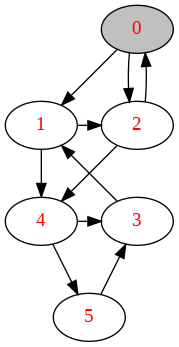
\includegraphics[width=0.2\columnwidth]{fig/depth_first_graph_search_process0.png}
    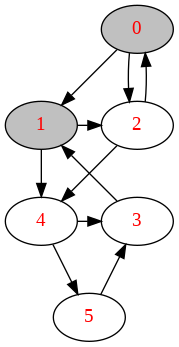
\includegraphics[width=0.2\columnwidth]{fig/depth_first_graph_search_process1.png}
    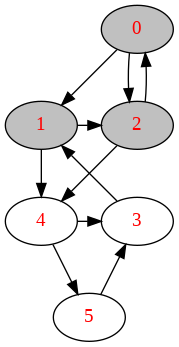
\includegraphics[width=0.2\columnwidth]{fig/depth_first_graph_search_process2.png}
    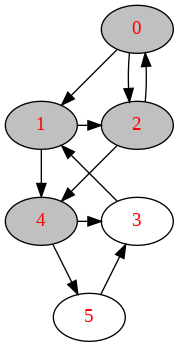
\includegraphics[width=0.2\columnwidth]{fig/depth_first_graph_search_process3.png}
    
     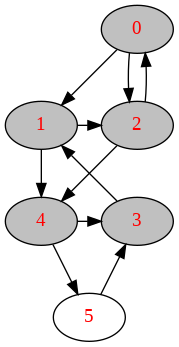
\includegraphics[width=0.2\columnwidth]{fig/depth_first_graph_search_process4.png}
    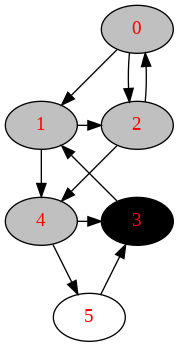
\includegraphics[width=0.2\columnwidth]{fig/depth_first_graph_search_process5.png}
    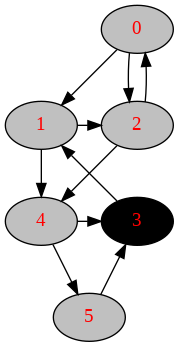
\includegraphics[width=0.2\columnwidth]{fig/depth_first_graph_search_process6.png}
    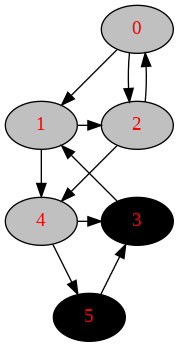
\includegraphics[width=0.2\columnwidth]{fig/depth_first_graph_search_process7.png}
    
        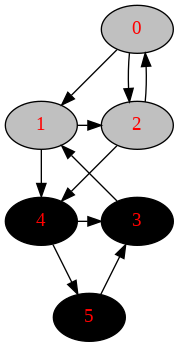
\includegraphics[width=0.2\columnwidth]{fig/depth_first_graph_search_process8.png}
    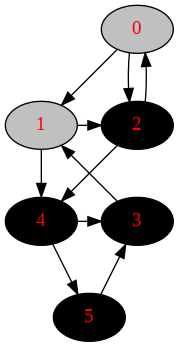
\includegraphics[width=0.2\columnwidth]{fig/depth_first_graph_search_process9.png}
    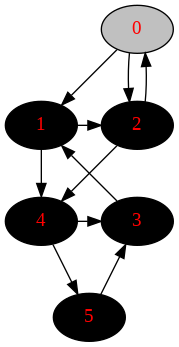
\includegraphics[width=0.2\columnwidth]{fig/depth_first_graph_search_process10.png}
    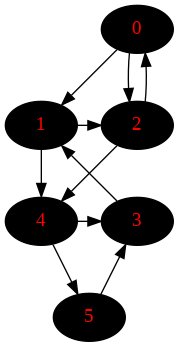
\includegraphics[width=0.2\columnwidth]{fig/depth_first_graph_search_process11.png}
    \caption{The process of Depth-first Graph Search. The black arrows denotes the the relation of $u$ and its not visited neighbors $v$. And the red arrow marks the backtrack edge. }
    \label{fig:depth_first_graph_search_process}
\end{figure}

As shown in Fig.~\ref{fig:depth_first_graph_search_process}, we
%Depth-first Search starts from a given source, and follows a single path in the graph to go as ``far'' as possible to visit unvisited nodes until (1) it meets a vertex that has no edge out; or (2) no unvisited adjacent vertices or say white vertices. Then it ``backtracks'' to its predecessor and start the above process again. DFS will discover all vertices that are reachable from the given source. 
start from 0, mark it gray, and visit its first unvisited neighbor 1, mark 1 as gray, and visit 1's first unvisited neighbor 2, then 2's unvisited neighbor 4, 4's unvisited neighbor 3.  For node 3, it does'nt have white neighbors, we mark it to be complete with black. Now, here, we ``backtrack'' to its predecessor, which is 4. And then we keep the process till 5 become gray. Because 5 has no edge out any more, it becomes black. Then the search backtracks to 4,  to 2, to 1, and eventually back to 0. We should notice the ordering of vertices become gray or black is different. From the figure, the gray ordering is \texttt{[0, 1, 2, 4, 3, 5]}, and for the black is \texttt{[3, 5, 4, 2, 1, 0]}. Therefore, it is necessary to distinguish the three states in the depth-first graph search at least. 


\paragraph{Three States Recursive Implementation} 
We add additional \texttt{colors} list to track the color of each vertices, \texttt{orders} to track the ordering of the gray, and \texttt{completed\_orders} for ordering vertices by their ordering of turning into black--when all of a node's neighbors become black which is after the recursive call in the code.  
\begin{lstlisting}[language = Python]
def dfs(g, s, colors, orders, complete_orders):
  colors[s] = STATE.gray
  orders.append(s)
  for v in g[s]:
    if colors[v] == STATE.white:
      dfs(g, v, colors, orders, complete_orders)
  colors[s] = STATE.black
  complete_orders.append(s)
  return
\end{lstlisting}
Now, we try to call the function with the undirected cyclic graph in Fig.~\ref{fig:graph_search_example}.
\begin{lstlisting}[language=Python]
v = len(ucg)
orders, complete_orders = [], []
colors = [STATE.white] * v
dfs(ucg,0, colors, orders, complete_orders)
\end{lstlisting}
Now, the \texttt{orders} and \texttt{complete\_orders} will end up differently:
\begin{lstlisting}[numbers=none]
[0, 1, 2, 4, 3, 5] [3, 5, 4, 2, 1, 0]
\end{lstlisting}

\paragraph{Edges}
\begin{figure}[!ht]
    \centering
       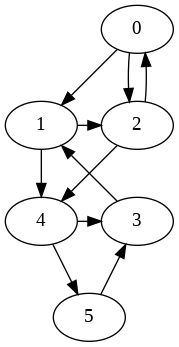
\includegraphics[width=0.33\columnwidth]{fig/directed_cyclic_graph_2.png}
     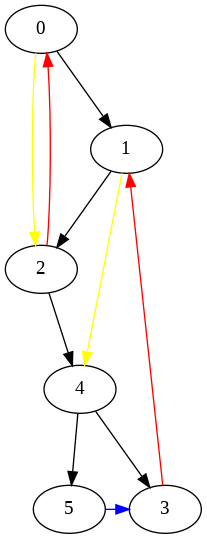
\includegraphics[width=0.28\columnwidth]{fig/depth_first_graph_search_edges(1).png}
    \caption{Classification of Edges: black, red, yellow, and blue marks tree edges, back edges, forward edges, and cross edges, respectively.}
    \label{fig:depth_first_graph_search_edges}
\end{figure}
Depth-first Graph Search on graph $G=(V, E)$ connects all reachable vertices from a given source in the graph in the form of  a depth-first forest $G_\pi$. Edges within $G_\pi$ are called \textbf{tree edges}. Tree edges are edges marked with black arrows in Fig.~\ref{fig:depth_first_graph_search_edges}. Other edges in $G$ can be classified into three categories based on Depth-first forest $G_\pi$, they are:
\begin{enumerate}
\item Back edges point from a node to one of its ancestors in the depth-first forest $G_\pi$. Marked as red edges in Fig.~\ref{fig:depth_first_graph_search_edges}.

\item Forward edges point from a node to one of its descendants in the depth-first forest $G_\pi$. Marked as yellow edges in Fig.~\ref{fig:depth_first_graph_search_edges}.

\item Cross edges point from a node to a previously visited node that is neither an ancestor nor a descendant in the depth-first forest $G_\pi$.  Marked as blue edges in Fig.~\ref{fig:depth_first_graph_search_edges}.
\end{enumerate}

Classification of edges provide important information about the graph, e.g. to if we detect a back edge in directed graph, we find a cycle.



\paragraph{Parenthesis Structure} In either undirected or directed graph, the discovered time when state goes from WHITE to GRAY and the finish time  when state turns to BLACK from GRAY has the parenthesis structure. We modify \texttt{dfs} to track the time:  a static variable \texttt{t} is used to track the time, \texttt{discover} and \texttt{finish} is used to record the first discovered and finished time. The implementation is shown:
\begin{lstlisting}[language=Python]
def dfs(g, s, colors):
  dfs.t += 1 # static variable
  colors[s] = STATE.gray
  dfs.discover[s] = dfs.t
  for v in g[s]:
    if colors[v] == STATE.white:
      dfs(g, v, colors)
  # complete
  dfs.t += 1
  dfs.finish[s] = dfs.t
  return
\end{lstlisting}
Now, we call the above function with directed graph in Fig.~\ref{fig:depth_first_graph_search_edges}.
\begin{lstlisting}[language=Python]
v = len(dcg)
colors = [STATE.white] * v
dfs.t = -1
dfs.discover, dfs.finish = [-1] * v, [-1] * v
dfs(dcg,0, colors)
\end{lstlisting}
The output for \texttt{dfs.discover} and \texttt{dfs.finish} are:
\begin{lstlisting}[numbers=none]
([0, 1, 2, 4, 3, 6], [11, 10, 9, 5, 8, 7])
\end{lstlisting}
From \texttt{dfs.discover} and \texttt{dfs.finish} list, we can generate a new list of merged order, \texttt{merge\_orders} that arranges nodes in order of there discovered and finish time. The code is as:
\begin{lstlisting}[language=Python]
def parenthesis(dt, ft, n):
  merge_orders = [-1] * 2 * n
  for v, t in enumerate(dt):
    merge_orders[t] = v
  for v, t in enumerate(ft):
    merge_orders[t] = v

  print(merge_orders)
  nodes = set()
  for i in merge_orders:
    if i not in nodes:
      print('(', i, end = ', ')
      nodes.add(i)
    else:
      print(i, '),', end = ' ')
\end{lstlisting}
The output is:
\begin{lstlisting}[language=Python]
[0, 1, 2, 4, 3, 3, 5, 6, 6, 5, 4, 2, 1, 0]
( 0, ( 1, ( 2, ( 4, ( 3, 3 ), ( 5, ( 6, 6 ), 5 ), 4 ), 2 ), 1 ), 0 ), 
\end{lstlisting}
We would easily find out that the ordering of nodes according to the discovery and finishing time makes a well-defined expression in the sense that the parentheses are properly nested.
\begin{bclogo}[couleur = blue!30, arrondi=0.1,logo=\bccrayon,ombre=true]{Questions to ponder: } 
\begin{itemize}
\item Implement the iterative version of the recursive code.
\end{itemize}
\end{bclogo}

%%%%%%%%%%%%%%%%BFS Graph Search%%%%%%%%%%%%%%
\subsection{Breadth-first Graph Search}
We can observe the visiting ordering of the nodes are exactly the same as the free tree. If we add one edge of the predecessor node and the current node, for example, at first, we start at 0, we add edges (0, 1) and (0, 2) in a tree structure. Next, we expand 1, which will have unvisited neighbors 3 and 4, we add edges (1, 3) and (1, 4). At the end, all of these tracked edges will form a tree, which is exactly the same as of the free tree in Fig.~\ref{fig:cyclic_graph_search_bfs}.  We call such tree a \textbf{Breath-first Search Tree}. The tree contains all vertices reachable from $s$, if we denote nodes as $V_t$ and the edges are from each node's predecessor to this node, denotes as $E_t = {(pi[V_t], V_t), V_t \neq s}$. The subgraph of $(V_t, E_t)$ is called the \textbf{Predecessor Subgraph}.  With the search tree, we can see that the paths between any two vertices are the shortest path that is defined by the length of a path, which clearly in the Depth-first Search Tree that is not the case. 
\subsection{Introduction} 
 Given a graph $G = (V, E)$, and a \textit{source} vertex $s$, the aim of Breadth-first search is to explore the edges of $G$ to discover all vertices that are reachable from the source $s$ just as the depth-first search. However, BFS visits vertices that are reachable from the source in the order of distance from the source. More specifically, let us use $d$ to denote the distance, in the example, we are given vertex $0$ as the source. And first, we visit its neighbors $1, 2$ since they are the closest ones among all the other vertices in the graph with $d=1$. The edge $(0, 1), (0, 2)$ are added to the BFS tree. Next, move to 0's first neighbor 1, and visited 1's unvisited neighbors, $3, 4$ with $d=2$.  The whole process is depicted in Fig.~\ref{fig:bfs_search}.  
 \begin{figure}[!ht]
    \centering
    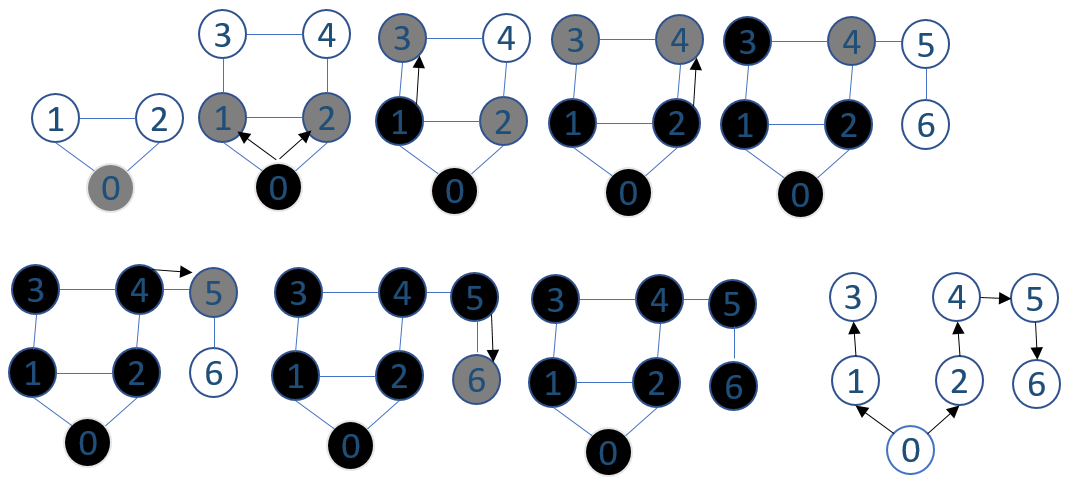
\includegraphics[width=0.9\columnwidth]{fig/bfs_example_1.png}
    \caption{The process of Breath-first-search. The black arrows denotes the the relation of $u$ and its not visited neighbors $v$. All these edges constructs a breath-first-tree. The visiting orders of BFS starting from vertex $0$ is [0, 1, 2, 3, 4, 5, 6].}
    \label{fig:bfs_search}
\end{figure}
\paragraph{Shortest Paths, Completeness, and Optimality}  The BFS strategy can produce the shortest-path from a source to any reachable vertex. This indicates that Breath-first graph search is \textbf{complete}: if there exists paths that can be reached from the source, we would find one of them--the shortest one. Thus, if our goal test is to find the shortest path to a target, we would find it at the distance $d_t$, which further  makes it \textbf{optimal}. While in the depth-first graph search, it is complete that we can find a reachable path, but it is not optimal. To be able to find the shortest path, we have to use the depth-first tree search to enumerate all possible acycle paths between the source and the target, only after then, we can compare all the candidates and get the shortest one,  which makes the complexity as large as $O(b^d)$ instead of in the case of bfs, which is $O(b^{d_t})$. 
 \begin{figure}[!ht]
    \centering
    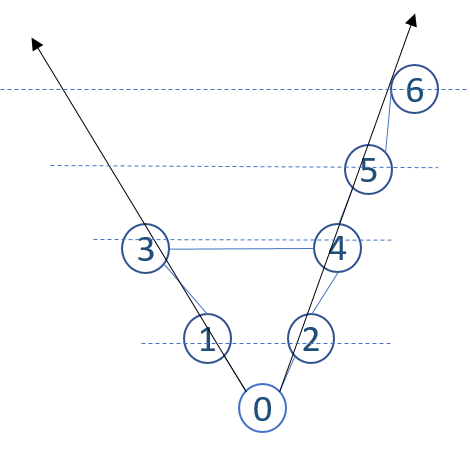
\includegraphics[width=0.3\columnwidth]{fig/bfs_shortest_dis.png}
    \caption{Visualize the BFS in level by level fashion.}
    \label{fig:bfs_search_shortest_path}
\end{figure}

\paragraph{Shortest Paths} To prove breath-first graph search generate a breath-first search where any  path between the root and other node is the shortest path evaluated in length. We can prove the correctness using mathematical induction. At first the frontier has only one node, the source, it is a path with length 0, which will be a trivial case. Next, we assume our frontier set has $n-1$ vertices, and $m$ nodes are still in exploring state, and all are the shortest paths to the source, the length of the exploring set to the source is $l_m$. Next, we just need to prove that the $m_u$ unvisited neighboring vertices of the $m$ exploring nodes makes the shortest path to the source. We can argue, because $m_u$ is not visited yet, thus they do not belong to the explored set or the frontiner set, making them impossible to have a path length as short as $l_m$. Because they are neighboring of the exploring nodes, which makes their path length to the source $l_m+1$, which is the minimum among all options. Breath-first graph search is indeed a greedy algorithm in the matter of the path length. We visualize this mathematical induction in Fig.~\ref{fig:bfs_search_shortest_path}. 


\subsubsection{Exploring}
Extend the tree traversal to the free tree. Before I give you all the definition and details about the graph search, let's explore together by extending the tree traversal to its equivalent free tree. 
\begin{figure}[!ht]
    \centering
    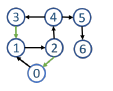
\includegraphics[width=0.4\columnwidth]{fig/free_tree_search.png}
     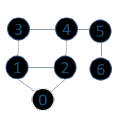
\includegraphics[width=0.4\columnwidth]{fig/cyclic_graph_searching.png}
    \caption{Left: A free tree, Right: A cyclic Graph}
    \label{fig:cyclic_graph_search}
\end{figure}
\paragraph{Free Tree Traversal} Assume the counterpart of recursive binary tree for the free tree shown in Fig.~\ref{fig:cyclic_graph_search} is a tree rooting at node 0, and if an internal node has only one child, say a left child. What is the output of preorder traversal? Represent the graph with adjacency list, and develop a recursive function that print out the same as the preorder traversal in the recursive tree. 

\paragraph{Analysis} First, we can just get the preorder traversal manually without coding, which will be [0, 1, 2, 4, 3, 5, 6]. Now, to develop a recursive traversal function in the free tree, we need to give our recursive function an argument to indicate which node to deal with in that function just as in the recursive tree traversal it takes a node. We set it as vertex number which starts at 0. Instead of call recursive function for the left and right child, in the free tree, it is replaced by checking its neighbors, and assume the neighbors are ordered by vertex number incrementally. The equivalent function will be:
\begin{lstlisting}[language=Python]
def recursive(g, vi):
  '''
  g: graph as an adjacency list
  vi: the vertex index
  '''
  print(vi, end=' ')
  for nv in g[vi]:   
    recursive(g, nv)
\end{lstlisting}
We call this function, it will have the exact output as the preorder traversal output.

\paragraph{Cycle} However, if we directly apply the above recursive function on the cyclic graph on the right side of Fig.~\ref{fig:cyclic_graph_search}, we will end up getting stack overflow error because we would meet  a cycle [0, 1, 2, 0]. In a graph, it is unavoidable to have cycles, that is why it is a graph and not a tree. So, how to avoid cycles? We know the definition of a cycle is a closed path that has has at least one node that repeats; in our failed run, it is 0. Therefore, let us add a \texttt{path} in the recursive function, and whenever we want to expand a node, we check if it forms a cycle or not by comparing the candidate with our path. 
\begin{lstlisting}[language=Python]
def recursive(g, vi, path):
  #print(path, end=' ')
  print(vi, end=' ')
  for nv in g[vi]:  
    if nv not in path: 
      recursive(g, nv, path+[nv])
\end{lstlisting}
Let's call it as \texttt{recursive(al, 0, [0])}, and the output that indicates the visiting order of vertices will be:
\begin{lstlisting}[numbers=none]
0 1 2 4 3 5 6 3 4 2 5 6 2 1 3 4 5 6 4 3 1 5 6 
\end{lstlisting}
 \begin{figure}[!ht]
    \centering
    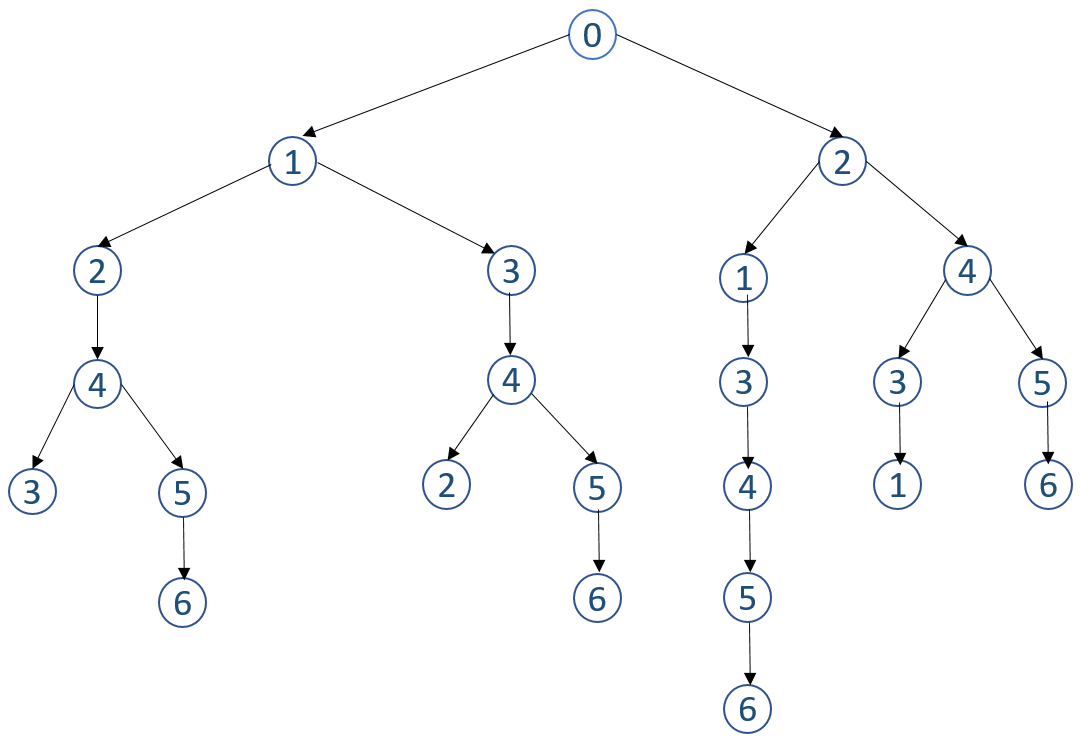
\includegraphics[width=0.9\columnwidth]{fig/depth_first_tree_search.png}
    \caption{The search tree using depth-first tree search }
    \label{fig:df_tree_search}
\end{figure}
\begin{figure}[!ht]
    \centering
    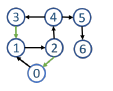
\includegraphics[width=0.5\columnwidth]{fig/free_tree_search.png}
    \caption{The search tree using depth-first graph search.}
    \label{fig:dfs_graph_search}
\end{figure}
And the following are all the paths comprise the search tree shown  in Fig.~\ref{fig:df_tree_search}.
\begin{lstlisting}[language=Python]
[0] [0, 1] [0, 1, 2] [0, 1, 2, 4] [0, 1, 2, 4, 3] [0, 1, 2, 4, 5] [0, 1, 2, 4, 5, 6] [0, 1, 3] [0, 1, 3, 4] [0, 1, 3, 4, 2] [0, 1, 3, 4, 5] [0, 1, 3, 4, 5, 6] [0, 2] [0, 2, 1] [0, 2, 1, 3] [0, 2, 1, 3, 4] [0, 2, 1, 3, 4, 5] [0, 2, 1, 3, 4, 5, 6] [0, 2, 4] [0, 2, 4, 3] [0, 2, 4, 3, 1] [0, 2, 4, 5] [0, 2, 4, 5, 6] 
\end{lstlisting}


\paragraph{Further Avoid Revisiting a Vertex} We see that from the above implementation, for a graph with only 7 nodes, we have been visiting nodes for 23 times. A lot of nodes have been repeating. 1 appears 3 times, 3 appears 4 times, and so on. As we see the visiting order being represented with a \texttt{search tree} in Fig.~\ref{fig:df_tree_search}, our complexity is getting close to $O(b^h)$, where $b$ is the branching factor and $h$ is the total vertices of the graph. If we simply want to search if a value exist in the graph or not, this is insanely complicating the situation. What we do next is to avoid revisiting the same vertex again and again, we conquer this by tracking the visiting state of a node. 
\begin{lstlisting}[language=Python]
def recursive(g, vi, visited):
  print(vi, end=' ')
  for nv in g[vi]:  
    if nv not in visited: 
      visited.add(nv)
      recursive(g, nv, visited)
\end{lstlisting}
Now, call the function as \texttt{recursive(al, 0, set([0]))}, the output is:
\begin{lstlisting}[numbers=none]
0 1 2 4 3 5 6 
\end{lstlisting}
Did you notice that this visiting order is the same as the ordering in the free tree!
\subsubsection{Introduction}
The last section actually gives us a very nice comprehensive peep at the variants of \textbf{depth-first search} in graph and its properties. 
\paragraph{Two Types of Depth-first Search in Graph} We have seen how to recursively search and avoids cycle or avoids revisiting nodes, these are two variants of DFS in graph:
\begin{enumerate}
    \item Depth-first Tree Search: If we recursively search as if our graph is a tree structure, this is called depth-first tree search. However, it is not \textbf{complete} because once we meet a cycle, it will never finishing checking all the vertices and the program will be eventually terminate due to stack overflow problem. We can resolve this cyclic issue by checking a vertex or a new state that is about to be expanded against with those on the path from the root to the current vertex: if it is a membership relation, we skip visiting this vertex to avoid cycle, making the search \textbf{complete}.
    \item Depth-first Graph Search: If we limit the search to only visit each vertex exactly once, which is complete and we would both avoid cycles and the redundant paths--for example, in the tree search version, we have path [0, 1, 3], [0, 2, 1, 3], [0, 2, 4, 3], and [0, 1, 2, 4, 3], there are multiple paths between the same two vertices 0 and 3. However, in the graph search, there is only one [0, 1, 2, 4, 3]. The graph search process, from one vertex to another forms an edge, we end up with a tree connecting all vertex of the graph, which is called \textbf{Depth-first Search Tree}. In our example, it is shown in Fig.~\ref{fig:dfs_graph_search} and is exactly the same as in Fig.\ref{fig:cyclic_graph_search}. 
\end{enumerate}
\paragraph{Completeness and Optimality} Both version of searching in graph can be complete, meaning if there exists one vertex that is what we are looking for, or a path that we need to find between a pair of vertices, we are sure we will find it.

However, both of them are \textit{nonoptimal}. For example, if the task is to find the shortest path from source 0 to target 2. The shortest path should be 0->2, however depth-first graph search will return 0->1->2. For the search tree using depth-first tree search, it can find the shortest path from source 0 to 2. However, it will explore the whole left branch starts from 1 before it finds its goal node on the right side. 

\paragraph{Time and Space Complexity} We have already discussed the depth-first tree search's complexity in the last chapter.  For the depth-first graph search, we use aggregate analysis. The search process covers all edges and vertices, which makes the time complexity as $O(|V|+|E|)$. For the space, it uses space $O(|V|)$ in the worst case to
store the stack of vertices on the current search path as well as the set of
already-visited vertices.

%%%%%%%%%%%%%%%%%%%%%%%%%%%%%%%Depth- first graph search%%%%%%%%%%%%%%%%%%%%%%%%%%%%%%%%%%%
\subsection{Depth-First Graph Search}
Further in this section, we focus  on Graph Search and discuss more advanced properties that might help us design graph algorithms. Let's see how the DFS process using BLACK, WHITE, and GREY state work. 

As shown in Fig.~\ref{fig:dfs_search_1}, we
%Depth-first Search starts from a given source, and follows a single path in the graph to go as ``far'' as possible to visit unvisited nodes until (1) it meets a vertex that has no edge out; or (2) no unvisited adjacent vertices or say white vertices. Then it ``backtracks'' to its predecessor and start the above process again. DFS will discover all vertices that are reachable from the given source. 
 \begin{figure}[!ht]
    \centering
    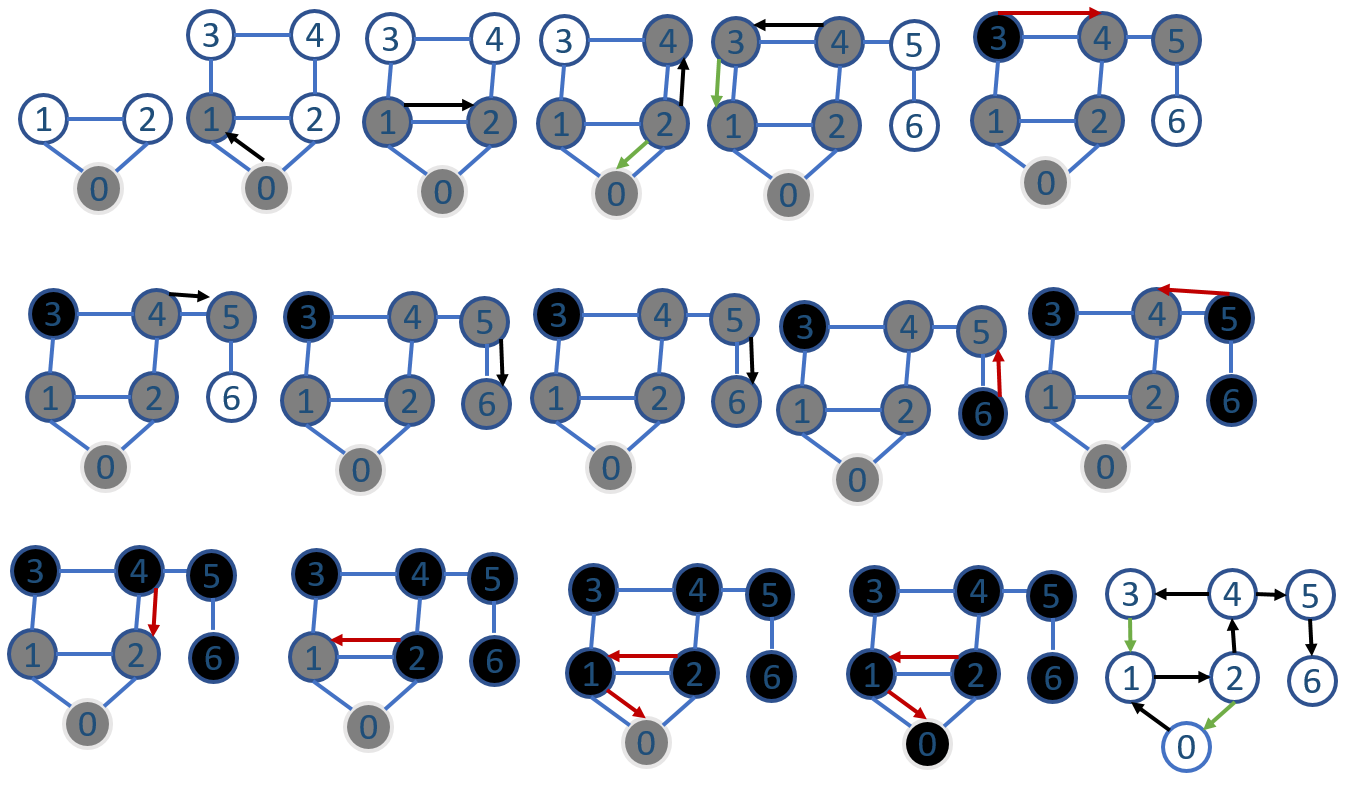
\includegraphics[width=0.9\columnwidth]{fig/dfs_procedure.png}
    \caption{The process of Depth-first-search. The black arrows denotes the the relation of $u$ and its not visited neighbors $v$. And the red arrow marks the backtrack edge. }
    \label{fig:dfs_search_1}
\end{figure}
start from 0, mark it gray, and visit its first unvisited neighbor 1, mark 1 as gray, and visit 1's first unvisited neighbor 2, then 2's unvisited neighbor 4, 4's unvisited neighbor 3. Then we are at the fifth and the sixth subgraph in the first row. Because for 3, it does'nt have white neighbors, we mark it to be complete with black. Now, here, we ``backtrack'' to its predecessor, which is 4. In this figure, red arrow marks the backtrack edges. And then we keep the process till 6 become gray. Because 6 has no edge out any more, the state will be complete. Then backtrack to 5, 5 become black, backtrack to 4, then to 2, to 1, and eventually back to 0. We should notice the ordering of vertices become gray or black is different. From the figure, the gray ordering is \texttt{[0, 1, 2, 4, 3, 5, 6]}, and for the black is \texttt{[3, 6, 5, 4, 2, 1, 0]}. Therefore, it is necessary to distinguish the three states in the depth-first graph search at least. 


\paragraph{Three states Recursive Implementation} We have already known how to implement DFS with \texttt{visited} to track the state, in this version, we want to track the three states. 
We add additional \texttt{colors} list to track the color of each vertices, \texttt{orders} to track the ordering of the gray, and \texttt{completed\_orders} for ordering vertices by their ordering of turning into black--when all of a node's neighbors become black which is after the recursive call in the code.  
\begin{lstlisting}[language = Python]
def dfs(g, s, colors, orders, complete_orders):
  colors[s] = STATE.gray
  orders.append(s)
  for v in g[s]:
    if colors[v] == STATE.white:
      dfs(g, v, colors, orders, complete_orders)
  colors[s] = STATE.black
  complete_orders.append(s)
  return
\end{lstlisting}
Now, we try to call the function with the same source of 0:
\begin{lstlisting}[language=Python]
v = len(al)
orders, complete_orders = [], []
colors = [STATE.white] * v
dfs(al,0, colors, orders, complete_orders)
\end{lstlisting}
Now, the \texttt{orders} and \texttt{complete\_orders} will end up differently:
\begin{lstlisting}[numbers=none]
[0, 1, 2, 4, 3, 5, 6] [3, 6, 5, 4, 2, 1, 0]
\end{lstlisting}

\subsubsection{Properties of Depth-first Graph Search}

\paragraph{Depth-first Search Tree} We have already defined the depth-first search tree which connects all reachable vertices from a given source in the graph in the form of a tree, where an edge is called \textit{tree edge}, which is the predecessor and successor, say it is $u$ and $v$ respectively. It can only be a tree edge if the color of $v$ is white when it is first explored in the search. A \textbf{back edge} $(u, v)$ is an edge that connects $v$ back to its predecessor $u$. \textcolor{red}{The condition is when the edge is explored, it will be an back edge if $u$ is  gray--meaning it is being explored but not done with all of its children. The back edge will have opposite direction compared with the tree edge, and they are where }.

\paragraph{Parenthesis Structure} In DFS, the discovered time and the finish time has the parenthesis structure. In our example, we use a static variable \texttt{t} of function \texttt{dfs} to track the time. \texttt{dt} and \texttt{ft} is used to record the first discovered and finished time. Now our dfs is defined as:
\begin{lstlisting}[language=Python]
def dfs(g, s, colors, dt, ft):
  dfs.t += 1 # static variable
  colors[s] = STATE.gray
  dt[s] = dfs.t
  for v in g[s]:
    if colors[v] == STATE.white:
      dfs(g, v, colors, dt, ft)
  dfs.t += 1
  ft[s] = dfs.t
  return
\end{lstlisting}
Now, we call the above function:
\begin{lstlisting}[language=Python]
v = len(al)
dt, ft = [-1] * v, [-1] * v
colors = [STATE.white] * v
dfs.t = -1
dfs(al,0, colors, dt, ft)
\end{lstlisting}
From the discover time and finish time list, we can generate a new list of merged order \texttt{merge\_orders} that arrange the node along the time. And we print out the node the first time it appears as `(v,' and second time as `v)'.
\begin{lstlisting}[language=Python]
def parenthesis(dt, ft, n):
  merge_orders = [-1] * 2 * n
  for v, t in enumerate(dt):
    merge_orders[t] = v
  for v, t in enumerate(ft):
    merge_orders[t] = v

  print(merge_orders)
  nodes = set()
  for i in merge_orders:
    if i not in nodes:
      print('(', i, end = ', ')
      nodes.add(i)
    else:
      print(i, '),', end = ' ')
\end{lstlisting}
The output is:
\begin{lstlisting}[language=Python]
[0, 1, 2, 4, 3, 3, 5, 6, 6, 5, 4, 2, 1, 0]
( 0, ( 1, ( 2, ( 4, ( 3, 3 ), ( 5, ( 6, 6 ), 5 ), 4 ), 2 ), 1 ), 0 ), 
\end{lstlisting}
We would easily find out that the ordering of nodes according to the discovery and finishing time makes a well-defined expression in the sense that the parentheses are properly nested.

\subsubsection{Iterative Implementation} 
In this book, we give two different versions of iterative implementations: (1) DFS, but not preserving the same discovering order (1) keep only the discovering order (2) keep both the discovering order and the finishing order. With these two iterative implementations, we have flexibility to pick one that work out the best. 
\paragraph{Method 1: Not preserving the discovering ordering}

The states that the node has first discovered last completed property, which means using a \texttt{stack} data structure we are able to implement iterative DFS.
For example, we first have stack $[0]$, then we put all of its unvisited vertices in $[1, 2]$, then we deal 2, and put all of 2's white neighbors in $[1, 2, 4]$, then 4, $[1, 2, 3, 5]$. Then 5, [1, 2, 3, 6]. Then it is 6, 3, 2, 1. Thereforce, the ordering of each vertex first in the stack is $[0, 1, 2, 4, 3, 5, 6]$. We have the following code:
\begin{lstlisting}[language=Python]
def dftIter(g, s):
  '''not preserving the same discovery ordering'''
  n = len(g)
  orders = []
  colors = [STATE.white] * n
  stack = [s]

  orders.append(s) # track gray order
  colors[s] = STATE.gray
        
  while stack:
    u = stack.pop()
    
    for v in g[u]:
      if colors[v] == STATE.white:
        colors[v] = STATE.gray
        stack.append(v)
        orders.append(v) # track gray order
    
  return orders
\end{lstlisting}
Run the above code with \texttt{dftIter(al, 1)}, we have ordering $[[1, 2, 3, 4, 5, 6, 0]$, which is different from the recursive DFS version $[[1, 2, 0, 4, 3, 5, 6]$. This is due to the different mechanism. To keep the same ordering of discovering order is not important. However, in our source code, we does provide a way to keep the same discovering ordering. 

\paragraph{Method 2: Preserving both Discover and Finish Ordering}
 Because in DFS each time, we start from $u$, we find one unvisited node  $u_1$ and move forward to find one unvisited node $u_2$ of $u_1$, until we met a node that has no unvisited adjacent nodes $v$. The visiting order will be $u, u_1, u_2,..., v$ , For this process, we use a \texttt{stack} to save these nodes, each time to append it at the end and this marks the state as gray, and each time visit the end node in the stack. In this process, there is no pop out from the stack. If we are at $v$, which can not move the path farther, this marks the state as black, and means the state is complete and this node is ready to be moved out of the stack.  Therefore, in the implementation,  a bool variable \texttt{bAdj} to check if we are able to find an unvisited node or not. If we can not find one, then we pop out, if we can, we break the loop because we just need one unvisited node.
\begin{lstlisting}[language = Python]
def dfsIter(g, s):
  '''iterative dfs'''
  v = len(g)
  orders, complete_orders = [], []
  colors = [STATE.white] * v
  stack = [s]

  orders.append(s) # track gray order
  colors[s] = STATE.gray
        
  while stack:
    u = stack[-1]
    bAdj = False
    for v in g[u]:
      if colors[v] == STATE.white:
        colors[v] = STATE.gray
        stack.append(v)
        orders.append(v) # track gray order
        bAdj = True
        break
     
    if not bAdj: # if no adjacent is found, pop out
      # complete
      colors[u] = STATE.black # this is not necessary in the code, just to help track the state
      complete_orders.append(u)
      stack.pop()
    
  return orders, complete_orders
\end{lstlisting}
Call \texttt{print(dfsIter(al, 0))}, the above code will have the same output as of the recursive implementation. 
\begin{lstlisting}[numbers=none]
([0, 1, 2, 4, 3, 5, 6], [3, 6, 5, 4, 2, 1, 0])
\end{lstlisting}









% As we have mentioned in Chapter~\ref{chapter_introduction_to_search}, there are generally three different searching strategies according to the orders in which nodes are expanded: breath-first search, depth-first search and priority-first search. In this section, we focus on the concepts instead of the exact implementation which varies to different data structures and will be detailed in the remaining sections. 

% Also, it is important to make clear of the concept of the tree-search and graph search. Tree search can happen on either a tree or a graph data structure.

% \paragraph{Tree Search on Tree Data Structure}  On the tree data structure, because there will be one and only one path between any two nodes in the tree, so normally we do not need to check the repeated nodes.

% \paragraph{Graph or Tree Search on Graph Data Structure} On the graph data structure, first, there might be more than one path between some two nodes in the graph. Second, there might have loop exist. Therefore, the common strategy in graph search is to use a set data structure to check repeated nodes, that is graph search will visit each node one and only once. The visiting order of the nodes can be connected as a search tree( that connects all $n$ vertexs with $n-1$ edges). This avoids the redundant paths and the loop.

% We  can also treat the graph as a tree, that the source node is a root, and any neighboring nodes will be children. In the graph, whenever to judge if a neighboring node is a child or not, we check if we have already visited this node from our path (it can not be our parent or grandparent node). So, this is a tree-search version on the graph data structure. 

\subsection{Breath-First Search in Graph} 
\subsubsection{Exploring} 
\begin{figure}[!ht]
    \centering
    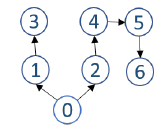
\includegraphics[width=0.4\columnwidth]{fig/bfs_free_tree.png}
     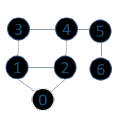
\includegraphics[width=0.4\columnwidth]{fig/cyclic_graph_searching.png}
    \caption{Left: A free tree, Right: A cyclic Graph}
    \label{fig:cyclic_graph_search_bfs}
\end{figure}
\paragraph{Free Tree Search} Similarly, we can smoothly translating the breath-first search in the recursive tree with queue into the free tree traversal. We need to choose a starting vertex in the free tree which is indeed a graph. The code is:
\begin{lstlisting}[language=Python]
def bfs(g, start):
  if not g:
    return 
  q = [start]
  while q:
    node = q.pop(0) # get node at the front of the queue
    print(node, end=' ')
    # Visist the neighbors
    for neig in g[node]:
      q.append(neig)
\end{lstlisting}
Now, calling the function with \texttt{start=0}, we have a visiting ordering of:
\begin{lstlisting}[numbers=none]
0 1 2 3 4 5 6 
\end{lstlisting}
\paragraph{Cycle} Move on to the same graph used in DFS. Same here, to avoid the \texttt{while} loop to hang and run forever, we need an approach to avoid cycle. If our purpose it to enumerate all acyclic paths in the graph, we won't try to use breath-first search, because in order to do so, for each node that goes into the queue, we need to save a corresponding longest path from start to that node, and it is a lot of extra memory compared with using DFS. 
\paragraph{Avoid Revisiting a Vertex} We follow the depth-first graph search where each vertex is only visited once. We use a \texttt{visited} set too. 
\begin{lstlisting}[language=Python]
def bfs(g, start):
  if not g:
    return 
  q = [start]
  visited = set([start])
  while q:
    node = q.pop(0) # get node at the front of the queue
    print(node, end=' ')
    # Visist the neighbors
    for neig in g[node]:
      if neig not in visited:
        visited.add(neig)
        q.append(neig)
\end{lstlisting}
The print out from calling the function with \texttt{start=0} and with the graph, we have:
\begin{lstlisting}[numbers=none]
0 1 2 3 4 5 6 
\end{lstlisting}
We can observe the visiting ordering of the nodes are exactly the same as the free tree. If we add one edge of the predecessor node and the current node, for example, at first, we start at 0, we add edges (0, 1) and (0, 2) in a tree structure. Next, we expand 1, which will have unvisited neighbors 3 and 4, we add edges (1, 3) and (1, 4). At the end, all of these tracked edges will form a tree, which is exactly the same as of the free tree in Fig.~\ref{fig:cyclic_graph_search_bfs}.  We call such tree a \textbf{Breath-first Search Tree}. The tree contains all vertices reachable from $s$, if we denote nodes as $V_t$ and the edges are from each node's predecessor to this node, denotes as $E_t = {(pi[V_t], V_t), V_t \neq s}$. The subgraph of $(V_t, E_t)$ is called the \textbf{Predecessor Subgraph}.  With the search tree, we can see that the paths between any two vertices are the shortest path that is defined by the length of a path, which clearly in the Depth-first Search Tree that is not the case. 
\subsection{Introduction} 
 Given a graph $G = (V, E)$, and a \textit{source} vertex $s$, the aim of Breadth-first search is to explore the edges of $G$ to discover all vertices that are reachable from the source $s$ just as the depth-first search. However, BFS visits vertices that are reachable from the source in the order of distance from the source. More specifically, let us use $d$ to denote the distance, in the example, we are given vertex $0$ as the source. And first, we visit its neighbors $1, 2$ since they are the closest ones among all the other vertices in the graph with $d=1$. The edge $(0, 1), (0, 2)$ are added to the BFS tree. Next, move to 0's first neighbor 1, and visited 1's unvisited neighbors, $3, 4$ with $d=2$.  The whole process is depicted in Fig.~\ref{fig:bfs_search}.  
 \begin{figure}[!ht]
    \centering
    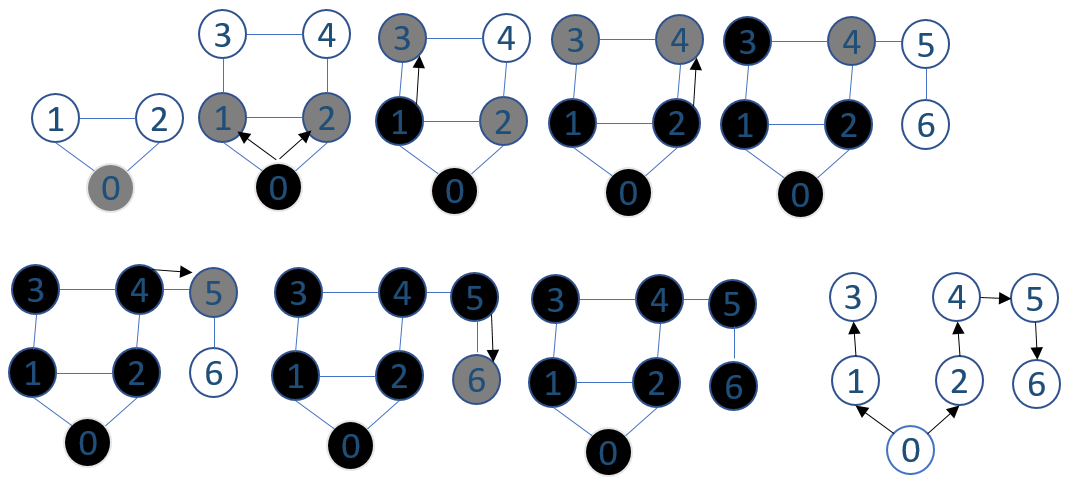
\includegraphics[width=0.9\columnwidth]{fig/bfs_example_1.png}
    \caption{The process of Breath-first-search. The black arrows denotes the the relation of $u$ and its not visited neighbors $v$. All these edges constructs a breath-first-tree. The visiting orders of BFS starting from vertex $0$ is [0, 1, 2, 3, 4, 5, 6].}
    \label{fig:bfs_search}
\end{figure}
\paragraph{Shortest Paths, Completeness, and Optimality}  The BFS strategy can produce the shortest-path from a source to any reachable vertex. This indicates that Breath-first graph search is \textbf{complete}: if there exists paths that can be reached from the source, we would find one of them--the shortest one. Thus, if our goal test is to find the shortest path to a target, we would find it at the distance $d_t$, which further  makes it \textbf{optimal}. While in the depth-first graph search, it is complete that we can find a reachable path, but it is not optimal. To be able to find the shortest path, we have to use the depth-first tree search to enumerate all possible acycle paths between the source and the target, only after then, we can compare all the candidates and get the shortest one,  which makes the complexity as large as $O(b^d)$ instead of in the case of bfs, which is $O(b^{d_t})$. 
 \begin{figure}[!ht]
    \centering
    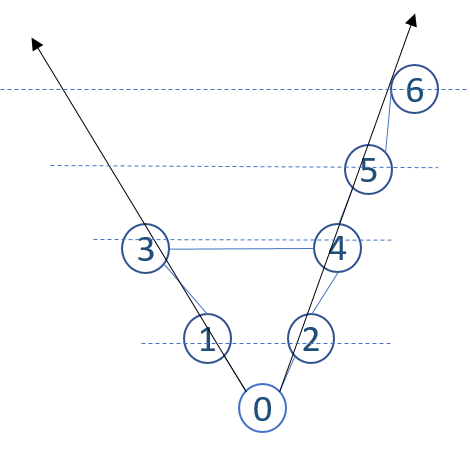
\includegraphics[width=0.3\columnwidth]{fig/bfs_shortest_dis.png}
    \caption{Visualize the BFS in level by level fashion.}
    \label{fig:bfs_search_shortest_path}
\end{figure}

\paragraph{Shortest Paths} To prove breath-first graph search generate a breath-first search where any  path between the root and other node is the shortest path evaluated in length. We can prove the correctness using mathematical induction. At first the frontier has only one node, the source, it is a path with length 0, which will be a trivial case. Next, we assume our frontier set has $n-1$ vertices, and $m$ nodes are still in exploring state, and all are the shortest paths to the source, the length of the exploring set to the source is $l_m$. Next, we just need to prove that the $m_u$ unvisited neighboring vertices of the $m$ exploring nodes makes the shortest path to the source. We can argue, because $m_u$ is not visited yet, thus they do not belong to the explored set or the frontiner set, making them impossible to have a path length as short as $l_m$. Because they are neighboring of the exploring nodes, which makes their path length to the source $l_m+1$, which is the minimum among all options. Breath-first graph search is indeed a greedy algorithm in the matter of the path length. We visualize this mathematical induction in Fig.~\ref{fig:bfs_search_shortest_path}. 

So far, we know we can get the shortest path, but how to print out the shortest paths between the source and other vertexs at the same time? In the DFS, path recording is more straightforward. In BFS, a similar way as of DFS is to track each node's all predecessors. Say we have \texttt{(n, [s, p\_1, p\_2, ..., p\_m]}. It is doable, programmingly speaking. But it is too costly, we are enlarging the space complexity by $d$ times, making it $O(|V|*d)$. A better way, that only adds $O(|V|)$ space is to only save all edges of the Breath-first search tree, not with edge list representation, but with a list where it is either indexed by predecessor or successor and valued by the other. So, which one to choose? Look at the BF tree, say if we want to get the shortest path between 0 and 5. If we start from 0, there are branches, that we need to search through all the nodes in order to find and reconstruct the path $(0\rightarrow 5)$. However, if we start at node 5, and  search in opposite direction, always track back its predecessor, we will eventually get to the source, where in our case is 0.  This is more efficient, thus the answer is we index our edge list by successor and value it by the predecessor. Let's name it as predecessor list \texttt{pl}, and we can remember this with \texttt{pl[s]=p}. We start the predecessor of the source vertex to be itself, which will has a length of 0. This predecessor can also be replaced by \texttt{dict} to enable random access. In addition, we add a distance list to track the distance of the shortest path from source to other nodes.  Now, our code looks like:
\begin{lstlisting}[language=Python]
def bfs_path(g, start):
  if not g:
    return 
  v = len(g)
  pl = [None] * v # Predecessor list
  dl = [0] * v # Distance list
  q = [start]
  visited = set([start])
  while q:
    node = q.pop(0)
    for neig in g[node]:
      if neig not in visited:
        pl[neig] = node
        dl[neig] = dl[node] + 1
        visited.add(neig)
        q.append(neig)
  
  return pl, dl
\end{lstlisting}
\paragraph{Print Shortest Path} To be able print the path of $s$ and $t$ we can start with $t$ and traverse back to $s$ through the predecessor. That is we first check out $t$'s predecessor if it has one, and then the predecessor's predecessor, and so on. There are two ways to do it: recursive and iterative.  

In the recursive solution, we first call \texttt{(s, t)}, and then \texttt{(s, pl[t])} to find its predecessor, and up till the base case where the source and the target is the same. Because we are visiting the path from source to target in reversed order, remember in the recursive function, there are always two passes: before the recursive call and after the recursive call. If we update \texttt{path} before the recursive call, we need to reverse the list, which can be avoid if we update it afterwards.
\begin{lstlisting}[language=Python]
def get_path(s, t, pl, path):
  if s == t:   
    pass
  elif pl[t] is None:
    print('no path from ', s, ' to ', t)
  else:
    get_path(s, pl[t], pl, path)   
  path.append(t)
  return
\end{lstlisting}
Now, with the example of \texttt{s=0, t=5}, we have the following output:
\begin{lstlisting}[numbers=none]
\end{lstlisting}

In the iterative solution, we use a \texttt{while} loop to visit the predecessor till we meet the source. The path will needed to reversed at the end.
\begin{lstlisting}[language=Python]
def get_path(s, t, pl):
  p = t
  path = []
  while p != s:
    path.append(p)
    p = pl[p]
  path.append(s)
  return path[::-1]
\end{lstlisting}

\begin{bclogo}[couleur = blue!30, arrondi=0.1,logo=\bccrayon,ombre=true]{Please implement breath-first-search that multiple start vertices are given? }
\end{bclogo}

\subsubsection{Complexity Analysis} Because in the process of BFS, each vertex is enqued and dequeued exactly one time, this process takes $O(|V|)$. Because at each iteration, it scans each edge exactly once too, this takes $O(|E|)$. Sums up we have the total time complexity of $O(|V|+|E|)$.

\paragraph{Time Complexity} the time complexity is bounded by the size of the state space, which is essentially a graph, which makes our complexity bound to be $O(|V|+|E|)$. A tighter bound of the time complexity of breath-first search is the same as its nodes in the search tree. Starting from root node, assume an uniform tree which has equal branch factor for all nodes $b$. The nodes at each level $i$ will be $b^i, i\in[0, d]$. Now, suppose that the solution is at depth $d$. In the worst case, it is the last node generated at $d$-th level. Then the total number of nodes is :
\begin{equation}
    \sum_{i=0}^{d} b^i = O(b^d)
\end{equation}

\paragraph{Space Complexity} For breath-first search, in some condition such in the graph, we need to keep two sets: \textit{explored set} and \textit{frontier list}. The space complexity gets maximum at the last level, where there will be $O(b^{d-1})$ nodes in the explored set and $O(b^d)$ nodes in the frontier. If it is a tree, we do not need to keep the explored set to avoid loops, therefore,  the space complexity comes from the space taken by the frontier list. An exponential complexity bound such as $O(b^d)$ is actually scary. 

(table time and memory requirements for breath-first search)

Two lessons can be learned from this given table. First, the memory requirements are a bigger problem for breath-first search than is the execution time. The second lesson is that time is still a major factor. If your problem has a solution at depth 16, then it will takes about 350 years for breath-first search to find it. Knowing the time complexity of search strategies can guide us to find more efficient algorithms to solve the real problems. 

 \subsubsection{Applications} The common problems that can be solved by BFS are those only need one solution: the best one such like getting the shortest path. As  we will learn later that breath-first-search is commonly used as archetype to solve graph optimization problems, such as Prim's minimum-spanning-tree algorithm and Dijkstra's single-source-paths algorithm.

%%%%%%%%%%%%%%%%%%%%%%%%%%%%Tree Traversal%%%%%%%%%%%%%%%%%%%%
\section{Tree Traversal}
\subsection{Depth-First Tree Traversal}
%\paragraph{Tree traversal for the rooted tree}
\begin{figure}[H]
    \centering
    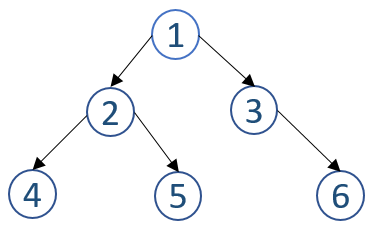
\includegraphics[width = .45\columnwidth]{fig/binary_tree_example.png}
    \caption{Exemplary Binary Tree }
    \label{fig:binary_tree_traversal_example}
\end{figure}
\subsubsection{Introduction}
% Let us see how we can iterate all nodes of the recursive tree we just constructed. 
Depth-first search starts at the root node and continues branching down a particular path; it selects a child node that is at the deepest level of the tree from the frontier to expand next and defers the expansion of this node's siblings. Only when the search hits a dead end (a node that has no child) does the search ``backtrack'' to its parent node, and continue to branch down to  other siblings that were deferred. A recursive tree can be traversed recursively. We print out the value of current node, then apply recursive call on the left and right node; by treating each node as a subtree, naturally a  recursive call to a  node can be  thought of handling the traversal of that subtree. The code is quite straightforward:

%The root node is like a queen, she sent out two assistants to traverse all provinces, and these two assistants further send out its sub  finish the tasks and to combine the result is what the queen herself needs to do. Let us write the following recursive traversal function and observe its output first:
\begin{lstlisting}[language=Python]
def recursive(node):
  if not node:
    return
  print(node.val, end=' ')
  recursive(node.left)
  recursive(node.right)
\end{lstlisting}
Now, we call this function with a tree as shown in Fig.~\ref{fig:binary_tree_traversal_example}, the output that indicates the traversal order is:
\begin{lstlisting}[language=Python]
1 2 4 5 3 6 
\end{lstlisting}

% As we see, all three types of traversal, the search process where we say search tree deepened as much as possible on each child before going visiting the next sibling, this is also called \textbf{depth-first search} and 

% \paragraph{Backing Implementation of Depth First Search}
%  We know that the recursion is implemented implicitly with call stack,

\subsubsection{Three Types of Depth-first Tree Traversal}
\begin{figure}[!ht]
    \centering
    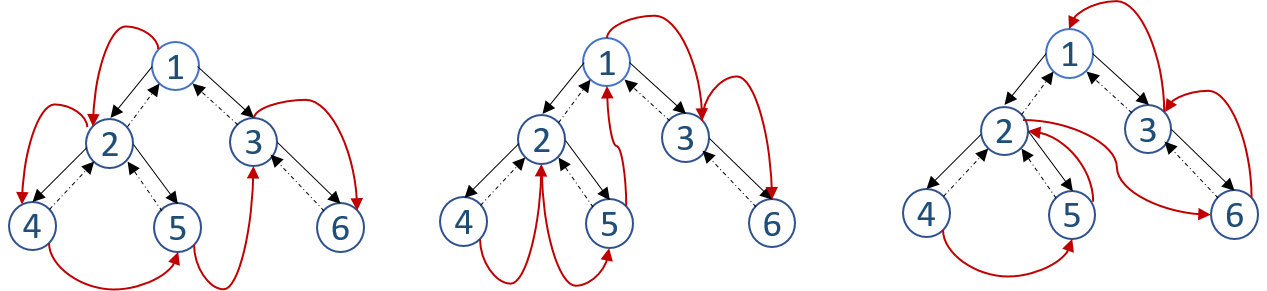
\includegraphics[width = .99\columnwidth]{fig/tree_traversal.png}
    \caption{Left: PreOrder, Middle: InOrder, Right: PostOrder. The red arrows marks the traversal ordering of nodes.}
    \label{fig:binary_tree_traversal}
\end{figure}
The visiting ordering between the current node, its left child, and its right child decides the following different types of recursive tree traversals: 

\begin{enumerate}[label=(\alph*)]
\item Preorder Traversal with ordering of  \texttt{[current node, left child, right child]}: it visits the nodes in the tree with ordering [1, 2, 4, 5, 3, 6].In our example, the recursive function first prints the root node 1, then goes to its left child, which prints out 2. Then it goes to node 4. From node 4, it next moves to its left child which is empty and leads to the termination of  the recursive call and then the recursion backward to node 4. Since node 4 has no right child, it further backwards to node 2, and then it check 2's right child 5. The same process of node 4 happens on node 5. It backwards to node 2, backwards to node 1, and keep visiting its right child 3, and the process goes on. We draw out this process in Fig.~\ref{fig:binary_tree_traversal}. 
\item Inorder Traversal with ordering of  \texttt{[left child, current node, right child]}: it traverses the nodes in ordering of [4, 2, 5, 1, 3, 6]. Three segments will appear with the inorder traversal for a root node: nodes in left subtree, root, and nodes in the right subtree.
\item Postorder Traversal with ordering of \texttt{[left child, right child, current node]}:  it traverses the nodes in ordering of [4, 5, 2, 6, 3, 1]. 
\end{enumerate}
We offer the code of Inorder Traversal:
\begin{lstlisting}[language=Python]
def inorder_traversal(node):
  if not node:
    return
  inorder_traversal(node.left)
  print(node.val, end=' ')
  inorder_traversal(node.right)
\end{lstlisting}




\begin{bclogo}[couleur = blue!30, arrondi=0.1,logo=\bccrayon,ombre=true]{Try to check  the other two orderings: \texttt{[left child, current node, right child]} and \texttt{[left child, right child, current node]} by hand first and then write the code to see if you get it right?} 
\end{bclogo}



\subsubsection{Return Values} 
Here, we want to do the task in a different way: We do not want to just print out the visiting orders, but instead write the ordering in a list and return this list. How would we do it? The process is the same, other than  we need to return something(not \texttt{None} which is default in Python). If we only have empty node, it shall return us an empty list \texttt{[]}, if there is only one node, returns \texttt{[1]} instead. 

Let us use PreOrder traversal as an example. To make it easier to understand, the same queen this time wants to do the same job in a different way, that she wants to gather all the data from these different states to her own hand. This time, she assumes the two generals A and B will return a \texttt{list} of the subtree, safely and sount. Her job is going to combine the list returned from the left subtree, her data, and the list returned from the right subtree. Therefore, the left general brings back $A=[2,4,5]$, and the right general brings back $B=[3, 6]$. Then the final result will be $queue + A + B = [1,2,4,5,3, 6]$. The Python code is given:
\begin{lstlisting} [language = Python]
def PreOrder(root):
    if root is None:
        return []
    ans = []
    left = PreOrder(root.left)
    right = PreOrder(root.right)
    ans = [root.val] + left + right
    return ans
\end{lstlisting}
\paragraph{An Example of Divide and Conquer} Be able to understand the returned value and combine them is exactly the method of \texttt{divide and conquer}, one of the fundamental algorithm design principles. This is a seemingly trivial change, but it approaches the problem solving from a totally different angle: atomic searching to divide and conquer that highlights the structure of the problem. The printing traversal and returning traversal represents two types of problem solving: the first is through searching--searching and treating each node more separately and the second is through reduce and conquer--reducing the problem to a series of smaller subproblems(subtrees where the smallest are empty subtrees) and construct the result by using the information of current problem and the solutions of the subproblems. 

\subsubsection{Complexity Analysis}
It is straightforward to see that it only visit all nodes twice, one in the forward pass and the other in the backward pass of the recursive call, making the time complexity linear to total number of nodes, $O(n)$. The other way is through the recurrence relation, we would write $T(n)=2\times T(n/2)+O(1)$, which gives out $O(n)$ too. 
% Similarly, the recursive code for the InOrder Traversal and PostTraversal:
% \begin{lstlisting}[language = Python]
% def InOrder(root):
%     if root is None:
%         return []
%     res = []
%     left = InOrder(root.left)
%     #print(root.val, end=',')
%     right = InOrder(root.right)
%     res =  left + [root.val]+ right
%     return res
    
% def PostOrder(root):
%     if root is None:
%         return []
%     res = []
%     left = PostOrder(root.left)
%     #print(root.val, end=',')
%     right = PostOrder(root.right)
%     res =  left + right + [root.val]
%     return res
% print(InOrder(root))
% print(PostOrder(root))
% # output 
% #[4, 2, 5, 1, 3]
% #[4, 5, 2, 3, 1]
% \end{lstlisting}
\subsection{Iterative Tree Traversal}
In Chapter Iteration and Recursion, we would know that the recursive function might suffer from the stack overflow, and in Python the recursion depth is $1000$. This section, we explore iterative tree traversals corresponding to PreOrder, InOrder, and PostOrder tree traversal. We know that the recursion is implemented implicitly with call stack, therefore in our iterative counterparts, they all use an explicit stack data structure to mimic the recursive behavior. 
\begin{figure}[!ht]
    \centering
    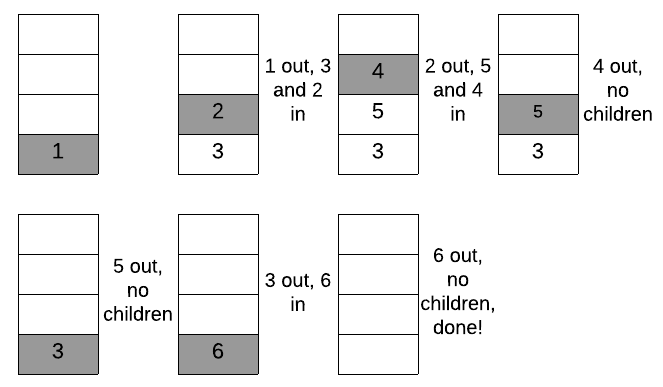
\includegraphics[width = .9\columnwidth]{fig/iterative_tree_traversal_preorder.png}
    \caption{The process of iterative preorder tree traversal.}
    \label{fig:iterative_tree_traveral_preorder}
\end{figure}

\paragraph{Simple Iterative Preorder Traversal} If we know how to implement a DFS iteratively with stack in a graph, we know our iterative preorder traversal. In this version, the stack saves all our frontier nodes. 
\begin{itemize}
    \item At first, we start from the root, and put it into the stack, which is 1 in our example.  
    \item  Our frontier set has only one node, thus we have to pop out node 1 and expand the frontiner set. When we are expanding node 1, we add its children into the frontier set by pushing them into the stack. In the preorder traversal, the left child should be first expanded from the frontier stack, indicating we should push the left child into the stack afterward the right child is pushed into. Therefore, we add node 3 and 2 into the stack. 
    \item We continue step 2.  Each time, we expand the frontier stack by pushing the toppest node's children into the stack and after popping out this node. This way, we use the first come last ordering of the stack data structure to replace the recursion.
\end{itemize}
We illustrate this process in Fig. ~\ref{fig:iterative_tree_traveral_preorder}.  The code is shown as:
\begin{lstlisting} [language = Python]
def PreOrderIterative(root):
    if root is None:
        return []
    res = []
    stack = [root]
    while stack:
        tmp = stack.pop()
        res.append(tmp.val)
        if tmp.right:
            stack.append(tmp.right)
        if tmp.left:
            stack.append(tmp.left)
    return res
\end{lstlisting}
%Even we know what is our main auxiliary data structure, we are no where close to the conversion. In the recursion, there are always two passes of visiting each state, while this is not the case of the iteration. 
\begin{figure}[!ht]
    \centering
    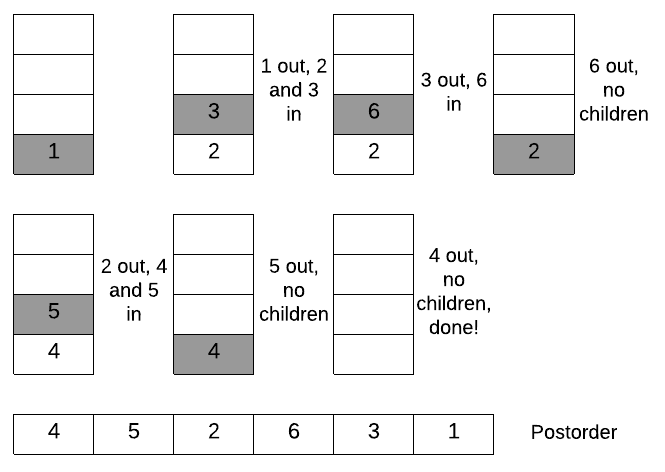
\includegraphics[width = .9\columnwidth]{fig/iterative_tree_traversal_postorder.png}
    \caption{The process of iterative postorder tree traversal.}
    \label{fig:iterative_tree_traveral_postorder}
\end{figure}

\paragraph{Simple Iterative Postorder Traversal} Similar to the above preorder traversal, the postordering is the ordering of nodes finishing the expanding of both its left and right subtree, thus with the ordering of  \texttt{left subtree}, \texttt{right subtree}, and \texttt{root}.   In preorder traversal,we obtained the ordering of  \texttt{root}, \texttt{left subtree}, and \texttt{right subtree}.  We try to reverse the ordering, it becomes \texttt{right subtree}, \texttt{left subtree}, and \texttt{root}.  This ordering only differs with postorder by a single a swap between the left and right subtree. So, we can use the same process as in the preorder traversal but expanding a node's children in the order of left and right child instead of right and left. And then the reversed ordering of items being popped out is the postoder traversal ordering. The process is shown in Fig.~\ref{fig:iterative_tree_traveral_postorder}. The Python implementation is shown as:
\begin{lstlisting}[language=Python]
def PostOrderIterative(root):
    if root is None:
        return []
    res = []
    stack = [root]
    while stack:
        tmp = stack.pop()
        res.append(tmp.val)
        if tmp.left:
            stack.append(tmp.left)
        if tmp.right:
            stack.append(tmp.right)
    return res[::-1]
\end{lstlisting}

\paragraph{General Iterative Preorder and Inorder Traversal } In the depth-first-traversal, we always branch down via the left child of the node at the deepest level in the frontier. The branching only stops when it can no longer find a left child for the deepest node in the frontier. Only till then, it will look around at expanding the right child of this deepest node, and if no such right child exists, it backtracks to its parents node and continues to check its right child to continue the branching down process. 

\begin{figure}[!ht]
    \centering
    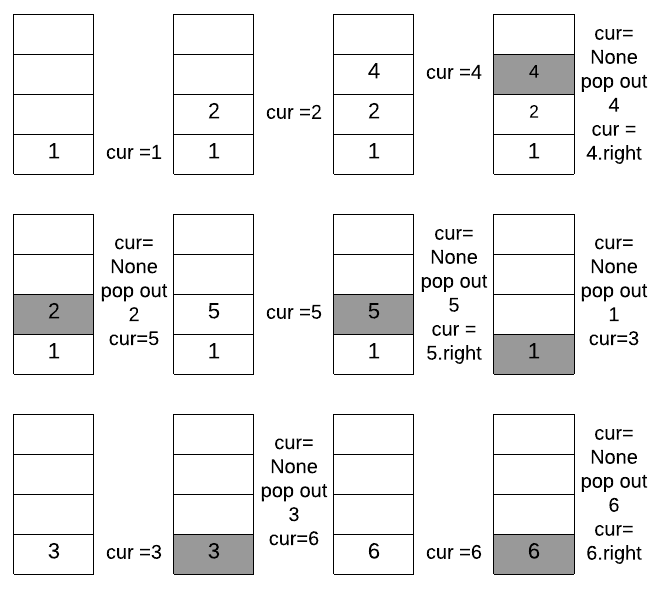
\includegraphics[width = .9\columnwidth]{fig/iterative_tree_traversal.png}
    \caption{The process of iterative tree traversal.}
    \label{fig:iterative_tree_traveral}
\end{figure}

Inspired by this process, we use a pointer, say \texttt{cur} to point to the root node of the tree, and we prepare an empty \texttt{stack}. The iterative process is:
\begin{itemize}
    \item The branching down process can be implemented with visiting  \texttt{cur} node, and pushing it into the \texttt{stack}. And then we set \texttt{cur=cur.left}, so that it keeps deepening down. 
    \item When one branch down process terminates, we pop out a node from \texttt{stack}, and we set \texttt{cur=node.right}, so that we expand the branching process to its right sibling. 
\end{itemize}
We illustrate this process in Fig.~\ref{fig:iterative_tree_traveral}. The ordering of items pushed into the stack is the preorder traversal ordering, which is [1, 2, 4, 5, 3, 6]. And the ordering of items being popped out of the stack is the inorder traversal ordering, which is [4, 2, 5, 1, 3, 6].  

\paragraph{Implementation} We use two lists--\texttt{preorders} and \texttt{inorders}--to save the traversal orders. The Python code is:
\begin{lstlisting}[language=Python]
def iterative_traversal(root):
  stack = []
  cur = root
  preorders = []
  inorders = []
  while stack or cur:
    while cur:
      preorders.append(cur.val)
      stack.append(cur)
      cur = cur.left
    node = stack.pop()
    inorders.append(node.val)
    cur = node.right
  return preorders, inorders
\end{lstlisting}


% \paragraph{Iterative PreOrder Traversal} Here is a common mistake we would make: we think we start at 1, put 1 in a stack, [1], then move to 2, have stack [1, 2], then move to 4, have a stack [1, 2, 4]. Now, 4 has no left child and no right child, we pop it out, and moves back to 2, then 2 would still have the left tree, which we end up with infinite loop. 
% \begin{lstlisting}[language=Python]
% def preorder_iter(root):
%   if not root:
%     return
%   stack = [root]
%   print(root.val, end=' ')
%   i = 0
%   while stack:
%     i += 1
%     if i==10:
%       return
%     node = stack[-1]
%     while node.left:
%       print(node.left.val, end=' ')
%       stack.append(node.left)
%       node = node.left
%     node = stack[-1]
%     if node.right:
%       print(node.right.val, end=' ')
%       stack.append(node.right)
%     else:
%       stack.pop()
% \end{lstlisting}
% We will end up with the print out:
% \begin{lstlisting}[numbers=none]
% 1 2 4 4 4 4 4 4 4 4 4 
% \end{lstlisting}
% This means when we are 


% \paragraph{PostOrder Iterative Tree Traversal} Need to explain better!!!
% \begin{lstlisting}[language = Python]
% def postorderTraversal(self, root):
%     if root is None:
%         return []
%     res = []
%     stack = [root]
%     while stack:
%         tmp = stack.pop()
%         res.append(tmp.val)
%         if tmp.left:
%             stack.append(tmp.left)
%         if tmp.right:
%             stack.append(tmp.right)
%     return res[::-1]
% \end{lstlisting}
% \paragraph{InOrder Iterative}. In the inorder, we need to print out all the left subtree first, and then the root, followed by the right. The process is as follows:
% \begin{lstlisting}
% 1) Create an empty stack S.
% 2) Initialize current node as root
% 3) Push the current node to S and set current = current->left until current is NULL
% 4) If current is NULL and stack is not empty then 
%       a) Pop the top item from stack.
%       b) Print the popped item, set current = popped_item->right 
%       c) Go to step 3.
% 5) If current is NULL and stack is empty then we are done. 
% \end{lstlisting}
% \begin{lstlisting}[language=Python]
% def InOrderIterative(root):
%     if root is None:
%         return []
%     res = []
%     stack = []
%     current = root
%     while current:
%         stack.append(current)
%         current = current.left
    
%     while stack:
%         tmp = stack.pop()
%         res.append(tmp.val)
%         current = tmp.right
%         while current:
%             stack.append(current)
%             current = current.left
        
%     return res
% \end{lstlisting}
% Another way to write this:
% \begin{lstlisting}[language=Python]
% def inorder(self, root):
%     cur, stack = root, []
%     while cur or stack:
%         while cur:
%             stack.append(cur)
%             cur = cur.left
%         node = stack.pop()
%         print(node.val)
%         cur = node.right
% \end{lstlisting}
% \begin{lstlisting}[language=Python]
% def inorder_iter(root):
%   if not root:
%     return
%   stack = []
%   node = root
%   i = 0
%   while stack or node:
%     print_stack(stack)
%     if node:
%       stack.append(node)
%       node = node.left
%     else:
%       node = stack.pop()
%       print(node.val, end = ' ')
%       node = node.right
% \end{lstlisting}

%%%%%%%%%%%BFS tree traversl%%%%%%%%%%%%%%
\subsection{Breath-first Tree Traversal}
\label{bfs_tree_traversal}
% \begin{figure}[!ht]
%     \centering
%     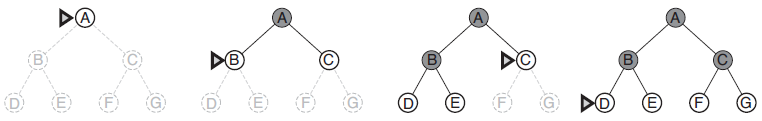
\includegraphics[width=0.96\columnwidth]{fig/general_breath_first_search.png}
%         \caption{Breath-first search on a simple search tree. At each stage, the node to be expanded next is indicated by a marker. }
%     \label{fig:breath_first_search_strategy}
% \end{figure}
\begin{figure}[H]
    \centering
    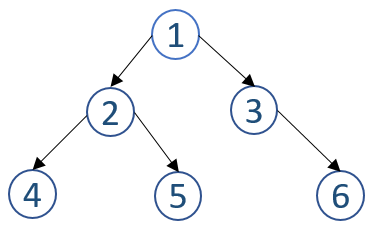
\includegraphics[width = .45\columnwidth]{fig/binary_tree_example.png}
    \caption{Draw the breath-first traversal order }
    \label{fig:binary_tree_traversal_example_bfs}
\end{figure}
Instead of traversing the tree recursively deepening down each time, the alternative is to visit  nodes level by level, as illustrated in Fig.~\ref{fig:fig:binary_tree_traversal_example_bfs} for our exemplary binary tree. We first visit the root node 1, and then its children 2 and 3. Next, we visit 2 and 3's children in order, we goes to node 4, 5, and 6.  This type of Level Order Tree Traversal uses the \textbf{breath-first search strategy} which differs from our covered depth-first search strategy. As we see in the example, the root node is expanded first, then all successors of the root node are expanded next, and so on, following a level by level ordering. We can also find the rule, the nodes first come and get first expanded. For example 2 is first visited and then 3, thus we expand 2's children first. Then we have 4 and 5. Next, we expand 3's children. This First come first expanded tells us we can rely on a queue to implement BFS. 




\paragraph{Simple Implementation} We start from the root, say it is our first level, put it in a list named \texttt{nodes\_same\_level}. Then we use a \texttt{while} loop, and each loop we visit all children nodes of \texttt{nodes\_same\_level} from the last level. We put all these children in a temporary list \texttt{temp}, before the loop ends, we assign \texttt{temp} to \texttt{nodes\_same\_level}, until the deepest level where no more children nodes will be found and leave our \texttt{temp} list to be empty and our while loop terminates. 
\begin{lstlisting}[language = Python]
def LevelOrder(root):
  if not root:
    return
  nodes_same_level = [root]
  while nodes_same_level:
    temp = []
    for n in nodes_same_level:
      print(n.val, end=' ')
      if n.left:
        temp.append(n.left)
      if n.right:
        temp.append(n.right)
    nodes_same_level = temp
\end{lstlisting}
The above will output  follows with our exemplary binary tree:
\begin{lstlisting}[language=Python]
1 2 3 4 5 6 
\end{lstlisting}

\paragraph{Implementation with Queue} As we discussed, we can use a FIFO queue to save the nodes waiting for expanding. In this case, at each \texttt{while} we only handle one node that are at the front of the queue. 
\begin{lstlisting}[language=Python]
def bfs(root):
  if not root:
    return
  q = [root]
  while q:
    node = q.pop(0) # get node at the front of the queue
    print(node.val, end=' ')
    if node.left:
      q.append(node.left)
    if node.right:
      q.append(node.right)
\end{lstlisting}






 
 
 %%%%%%%%%%%%%%%%%%%%%%%%%%%%%%%%%%Hands on examples%%%%%%%%%%%%%%%%%%%%%%%%%%%%%%
 \subsection{Hands-on Examples}
 
 \subsubsection{Get a more straightforward example} Add an example



% If we model each element in the array as a node in the graph, and assume given node $\mu$ with index $i$, if the element $v$ with index $j$, $j > i$,   is larger than $\mu$, there will be an edge $\mu \rightarrow v$. We draw the graph shown in Fig.~\ref{fig:tree_lis}.  The problem is modeled as finding the longest path in the graph, which can be solved with either DFS or BFS.  

% We define \texttt{curlen} as the length of increasing sequence from start node $[]$ to the current node, which can have $-\infty$ as value. length up. For example, at the leftmost node $101$, $curlen=2$ and the lowest $101$ node will have $curlen=4$ which is our longest LIS. Therefore, we would need a global variable $maxlen$ to track the maximum LIS. 

% \paragraph{Depth-first Graph Search} The implementation of Python is provided:
% \begin{lstlisting}[language=Python]
% import sys
    
% def dfs(curIdx, preV, curlen, a, maxlen):
  
%   for i in range(curIdx+1, len(a)):
%     # if a condition is satisfied, move to that node instead
%     if a[i] > preV:
%       dfs(i, a[i], curlen+1, a, maxlen)
%       maxlen[0] = max(maxlen[0], curlen+1)
%   return 
% \end{lstlisting}
% Now, we need to call the function with \texttt{curIdx=-1} and \texttt{preV=-sys.maxsize}, and \texttt{curlen=0} for the root node in the graph. 

% \paragraph{Breath-first Graph Search} The implementation of Python is provided:
% \begin{lstlisting}[language=Python]
% def bfs( nums):
%     """
%     :type nums: List[int]
%     :rtype: int
%     """
%     maxlen = 0
%     q = [(-1, -sys.maxsize, 0)] # start pos can be any number in nums
%     while q:
%       new_q = []
%       for idx, prev, curlen in q:
%         # search for number that is larger that current
%         for j in range(idx+1, len(nums)):
%           if nums[j] > prev: 
%             maxlen = max(maxlen, curlen + 1)
%             new_q.append((j, nums[j], curlen + 1))
%       q = new_q
%     return maxlen
% \end{lstlisting}
\subsubsection{Triangle (L120)} 
Given a triangle, find the minimum path sum from top to bottom. Each step you may move to adjacent numbers on the row below.
\begin{lstlisting}[numbers=none]
Example:
Given the following triangle:

[
[2],
[3,4],
[6,5,7],
[4,1,8,3]
]
The minimum path sum from top to bottom is 11 (i.e., 2 + 3 + 5 + 1 = 11).
\end{lstlisting}

  
\paragraph{Analysis}
Solution: first we can use dfs traverse as required in the problem, and use a global variable to save the minimum value. The time complexity for this is $O(2^n)$. When we try to submit this code, we get LTE error. The code is as follows:
\begin{lstlisting}[language = Python]
import sys
def min_path_sum(t):
  '''
  Purely Complete Search
  '''
  min_sum = sys.maxsize
  def dfs(i, j, cur_sum):
    nonlocal min_sum
    # edge case
    if i == len(t) or j == len(t[i]):
      # gather the sum
      min_sum = min(min_sum, cur_sum)
      return
    # only two edges/ choices at this step
    dfs(i+1, j, cur_sum + t[i][j])
    dfs(i+1, j+1, cur_sum + t[i][j])
  dfs(0, 0, 0)
  return min_sum
\end{lstlisting}





\subsection{Categorization}
So far we have covered the most important searching strategies, mainly two types: Uninformed and Informed (Heuristic) searches. DFS, DFS, Bidirectional search in the uninformed search group. 
\subsubsection{Explicit Search and Implicit Search}
\subsubsection{Complete Search and }
\subsubsection{exhaustive search and heuristic search}

\subsubsection{Applications}

An animation of DFS is available \url{https://www.cs.usfca.edu/~galles/visualization/DFS.html}
% The output will be $1, 2, 4, 6, 3, 5$. The path of the DFS actually composes a tree, we can this a \textbf{DFS tree}.

% In the code snipet, line 5 is to check if the current neighbor is visited or not. We can either use a SET or a list of Booleans, or if we know the total vertices are within 32 or 64, we can use bit as shown in Section~\ref{chapter_bit_section_bitwise}. 




\subsection{Comparison of BFS and DFS}
BFS and DFS is the most basic complete search in graph. They both search all vertices and edges by once, which made them share the same time complexity $O(|V|+|E|)$. We see, in the BFS, saving nodes of the gray state or black state has the same visiting ordering. Breadth-first search usually serves to find shortest path distances (and the associated predecessor subgraph) from a given source. Depth-first search is often a subroutine in another algorithm, as we shall see later in this chapter.
\section{Discussion of Graph Search}
\label{graph_types}
As we will in the future chapters, basic BFS and DFS lays the fundations of all graph and tree-based search. Understanding the properties of graph search throughly in this chapter will ease our journey to explore more advanced graph algorithms. 
There are some properties related to graph that we need to learn before moving to the advanced algorithms.

\paragraph{Completeness}
In the context of search, a complete algorithm is one that guarantees that if a path to the goal exists, the algorithm will reach the goal. Note that \textit{completeness} does not imply \textit{optimality} of the found path.

For example, breadth-first search (BFS) is complete (and in fact optimal if step costs are identical at a given level), because it can find all paths starting from a given source vertex in the graph. (This might not be the case if step cost at a given level is not identical). while depth-first search (DFS) on trees is incomplete (consider infinite or repeated states).

\begin{enumerate}
    \item How to check if a graph is connected? A: We can check if a graph is connected by starting at an arbitrary node and finding out if we can reach all other nodes. (Both DFS and BFS works)
    \item How to find cycle in a graph? A: A graph contains a cycle if during a graph search, we find a node whose neighbor has already been visited that marked as gray.
    \item How to check if a graph is bipartite? A: A graph is bipartite if its nodes can be colored using two colors so that there are
no adjacent nodes with the same color. It is surprisingly easy to check if a graph
is bipartite using graph traversal algorithms.
The idea is to color the starting node blue, all its neighbors red, all their
neighbors blue, and so on. If at some point of the search we notice that two
adjacent nodes have the same color, this means that the graph is not bipartite.
Otherwise the graph is bipartite and one coloring has been found. Note that in the general case, it is difficult to find out if the nodes in a graph
can be colored using k colors so that no adjacent nodes have the same color. Even
when k Æ 3, no efficient algorithm is known but the problem is NP-hard.
\end{enumerate}
\subsection{Coding Practice}
\paragraph{Property of Graph}
\begin{enumerate}
    \item 785. Is Graph Bipartite? (medium)
    \item 261. Graph Valid Tree (medium) 
    \item 797. All Paths From Source to Target(medium)
\end{enumerate}

\section{Informed Search Strategies**}
%%%%%%%%%%%%%%%%BFS%%%%%%%%%%%%%%%%%%%%%%%%%%%%%%
\subsection{Best-first Search}
 Best-first search is a search algorithm which explores a graph by expanding the most promising node  chosen according to a specified rule. The degree of promising of a node is described by a \textbf{heuristic evaluation function $f(n)$} which, in general, may depend on the description of the node $n$, the description of the goal, and the information gathered by the search up to that point, and most important, on any extra knowledge about the problem domain. 
 
 Breath-first search fits as  a special case in Best-first search if the objective of the problem is to find the shortest path from source to other nodes in the graph; it uses the estimated distance to source as a heuristic function.  At the start, the only node in the frontier set is the source node, expand this node and add all of its unexplored neighboring nodes in the frontier set and each comes with distance 1. Now, among all nodes in the frontier set, choose the node that is the most promising to expand. In this case, since they all have the same distance, expand any of them is good. Next, we would add nodes that have $f(n)=2$ in the frontier set, choose any one that has smaller distance. 
 
 A Generic best-first search will need a priority queue to implement instead of a FIFO queue used in the breath-first search. 
\end{document}